% !TEX root = ../main.tex
% 本文件由 build-tex.sh 从 12-DSP指南-第12章中译.md 生成，改内容请改 md 后重新生成

\chapter{快速傅里叶变换}\label{ch-12}

计算离散傅里叶变换（DFT）的方法有好几种，比如解联立线性方程组，或者第 8
章介绍的相关法。快速傅里叶变换（Fast Fourier Transform，FFT）是计算 DFT
的另一种方法。它得到的结果与其他方法相同，但效率高得惊人，计算时间常常能缩短几百倍。这就像坐喷气式飞机和走路的差别！如果没有
FFT，本书介绍的许多技术都没法实用。FFT 虽然只需要几十行代码，却是 DSP
中最复杂的算法之一。不过别泄气！你完全可以直接使用现成的 FFT
程序，而不必彻底弄懂它的内部原理。

\section{用复数 DFT 计算实数 DFT}

J.W. Cooley 和 J.W. Tukey 被公认为把 FFT
带给世界的人，他们的论文是：``An algorithm for the machine calculation
of complex Fourier
Series''（一种用机器计算复数傅里叶级数的算法），Mathematics
Computation，第 19 卷，1965 年，第 297～301
页。回头来看，其他人早在许多年前就发现了这一技术。例如，伟大的德国数学家卡尔·弗里德里希·高斯（1777--1855）一个多世纪以前就用过这种方法。这些早期工作基本被遗忘了，因为当时缺少让它变得实用的工具：数字计算机。Cooley
和 Tukey 之所以享有盛誉，是因为他们在正确的时间发现了
FFT------计算机革命的开端。

FFT 基于复数 DFT(complex DFT)，它是前四章讨论的实数 DFT(real DFT)
的一个更复杂的版本。这两种变换按各自表示数据的方式命名，也就是用复数还是用实数。``复数''(complex)
这个词并不是说这种表示方法困难或复杂，而是说它用到了一种特定的数学。复数数学确实常常困难又复杂，但名字不是从这儿来的。第
29 章讨论复数 DFT，并提供理解 FFT
算法细节所需的背景知识。本章的主题要简单些：怎样用 FFT 来计算实数
DFT，而不陷进高深数学的泥潭。

\begin{quote}
\textbf{译注：} 原书本章两处提到''第 29 章''讲复数 DFT，实际是第 31
章《复数傅里叶变换》（第 29 章是《DSP 上手实践》）。
\end{quote}

\begin{figure}[htbp]
\centering
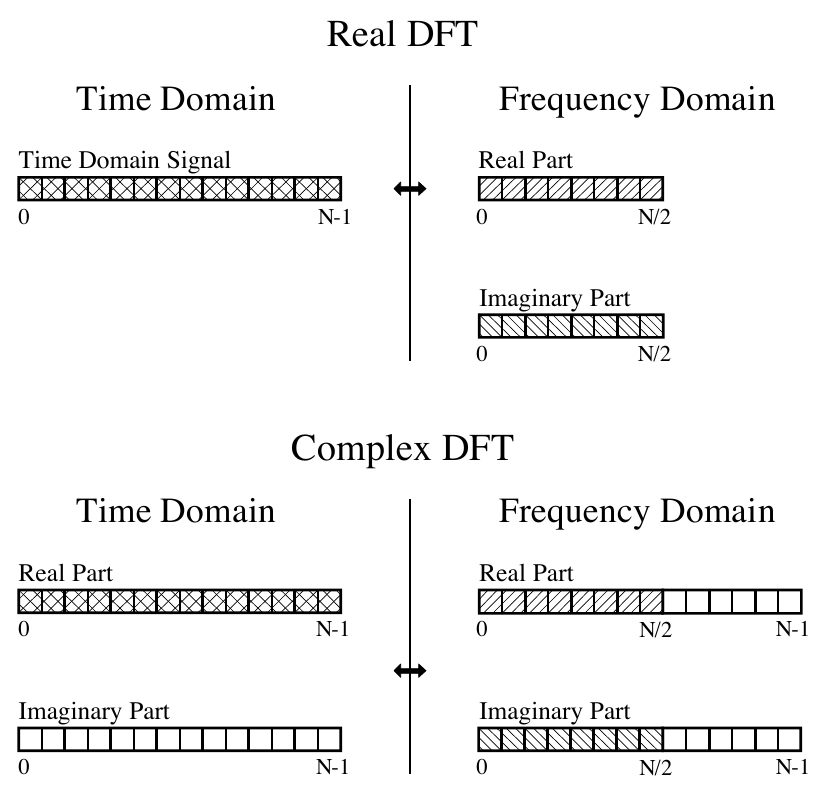
\includegraphics[width=0.688\linewidth,height=0.8\textheight,keepaspectratio]{assets/ch12/fig12-01.png}
\caption*{\textbf{图 12-1　实数 DFT 与复数 DFT 的比较。} 实数 DFT 把一个 N
点时域信号变成两个 N/2+1 点的频域信号。复数 DFT 把两个 N
点时域信号变成两个 N 点频域信号。画了斜线的区域表示两种变换共有的数值。
（Real DFT = 实数 DFT，Complex DFT = 复数 DFT；Time Domain =
时域，Frequency Domain = 频域；Time Domain Signal = 时域信号，Real Part
= 实部，Imaginary Part = 虚部。）}
\end{figure}

既然 FFT 是计算复数 DFT 的算法，弄清楚怎样把实数 DFT
的数据转入和转出复数 DFT 的格式就很重要。图 12-1 比较了实数 DFT 和复数
DFT 存放数据的方式。实数 DFT 把一个 N 点时域信号变换成两个 N/2+1
点的频域信号。这个时域信号就叫时域信号；频域中的两个信号分别叫实部(real
part)和虚部(imaginary
part)，存放余弦波和正弦波的幅度。这些在前几章都应该很熟悉了。

相比之下，复数 DFT 把两个 N 点时域信号变换成两个 N
点频域信号。两个时域信号也叫实部和虚部，和频域信号一样。尽管名字如此，这些数组中的所有值都只是普通的数。（如果你熟悉复数：数组值里不包含
j，j 是数学表达式的一部分。回忆一下，算子 Im( ) 返回的是一个实数。）

假设你有一个 N 点信号，需要借助复数 DFT（比如用 FFT 算法）来计算实数
DFT。首先，把这个 N 点信号放进复数 DFT
时域的实部，再把虚部的所有采样设为零。计算复数 DFT
后，频域得到一个实部信号和一个虚部信号，各有 N 个点。这两个信号的第
0～N/2 个采样，就对应实数 DFT 的频谱。

第 10 章讲过，把负频率包括进来时，DFT 的频域是周期性的（见图
10-9）。选哪一个周期是任意的，可以选 −1.0 到 0、−0.5 到 0.5、0 到
1.0，或者以采样率为参照的任何其他一个单位长的区间。复数 DFT 的频谱按 0
到 1.0 的方式包含负频率。也就是说，一个完整周期从第 0 个采样延伸到第 N−1
个采样，对应采样率的 0 到 1.0 倍。正频率位于第 0 到 N/2 个采样之间，对应
0 到 0.5。其余采样，即第 N/2+1 到 N−1 个，存放负频率的值（通常被忽略）。

用复数逆 DFT 计算实数逆 DFT
稍微难一点，因为你要保证负频率按正确的格式装入。记住，复数 DFT 的第
0～N/2 点与实数 DFT 相同，实部虚部都是如此。对于实部，第 N/2+1 点与第
N/2−1 点相同，第 N/2+2 点与第 N/2−2 点相同，依此类推，一直到第 N−1
点与第 1 点相同。虚部也是同样的基本模式，只是符号相反：第 N/2+1 点是第
N/2−1 点的相反数，第 N/2+2 点是第 N/2−2 点的相反数，等等。注意，第 0
点和第 N/2 点在这种复制模式中没有配对的点。可以参照图 10-9
来理解这种对称性。实际操作时，把实数 DFT 的频谱装入复数 DFT 数组的第
0～N/2 个采样，再用一个子程序生成第 N/2+1 到 N−1 个采样之间的负频率。表
12-1 就是这样一个程序。要检查对称性是否正确，可以在做完逆 FFT
后看时域的虚部：如果一切正确，它将全是零（用单精度计算时，会有百万分之几的噪声）。

\textbf{表 12-1}（注释已译成中文）

\begin{Shaded}
\begin{Highlighting}[]
\NormalTok{6000 \textquotesingle{}NEGATIVE FREQUENCY GENERATION}
\NormalTok{6010 \textquotesingle{}本子程序由实数频域生成复数频域。}
\NormalTok{6020 \textquotesingle{}进入本子程序时，N\% 是信号的点数，}
\NormalTok{6030 \textquotesingle{}REX[ ] 和 IMX[ ] 的第 0 到 N\%/2 个采样存放实数频域。}
\NormalTok{6040 \textquotesingle{}返回时，REX[ ] 和 IMX[ ] 的第 0 到 N\%{-}1 个采样存放复数频域。}
\NormalTok{6050 \textquotesingle{}}
\NormalTok{6060 FOR K\% = (N\%/2+1) TO (N\%{-}1)}
\NormalTok{6070 REX[K\%] = REX[N\%{-}K\%]}
\NormalTok{6080 IMX[K\%] = {-}IMX[N\%{-}K\%]}
\NormalTok{6090 NEXT K\%}
\NormalTok{6100 \textquotesingle{}}
\NormalTok{6110 RETURN}
\end{Highlighting}
\end{Shaded}

\textbf{C 实现}（完整可编译版本见
\texttt{c/table12-1\_negative\_freq.c}，其中用相关法复数 DFT
做对照，并按上文的方法检查逆变换后虚部是否为零）：

\begin{Shaded}
\begin{Highlighting}[]
\CommentTok{/* 6000：由实数频域生成复数频域。进入时 rex/imx 的 0～n/2 点有效，返回时 0～n{-}1 点都有效 */}
\DataTypeTok{static} \DataTypeTok{void}\NormalTok{ negative\_frequency\_generation}\OperatorTok{(}\DataTypeTok{double} \OperatorTok{*}\NormalTok{rex}\OperatorTok{,} \DataTypeTok{double} \OperatorTok{*}\NormalTok{imx}\OperatorTok{,} \DataTypeTok{int}\NormalTok{ n}\OperatorTok{)}
\OperatorTok{\{}
    \ControlFlowTok{for} \OperatorTok{(}\DataTypeTok{int}\NormalTok{ k }\OperatorTok{=}\NormalTok{ n }\OperatorTok{/} \DecValTok{2} \OperatorTok{+} \DecValTok{1}\OperatorTok{;}\NormalTok{ k }\OperatorTok{\textless{}=}\NormalTok{ n }\OperatorTok{{-}} \DecValTok{1}\OperatorTok{;}\NormalTok{ k}\OperatorTok{++)} \OperatorTok{\{}  \CommentTok{/* 6060：遍历负频率的每个点 */}
\NormalTok{        rex}\OperatorTok{[}\NormalTok{k}\OperatorTok{]} \OperatorTok{=}\NormalTok{ rex}\OperatorTok{[}\NormalTok{n }\OperatorTok{{-}}\NormalTok{ k}\OperatorTok{];}                    \CommentTok{/* 6070：实部偶对称 */}
\NormalTok{        imx}\OperatorTok{[}\NormalTok{k}\OperatorTok{]} \OperatorTok{=} \OperatorTok{{-}}\NormalTok{imx}\OperatorTok{[}\NormalTok{n }\OperatorTok{{-}}\NormalTok{ k}\OperatorTok{];}                   \CommentTok{/* 6080：虚部奇对称 */}
    \OperatorTok{\}}
\OperatorTok{\}}
\end{Highlighting}
\end{Shaded}

运行结果（N=64 随机实信号）：补出的负频率与完整频谱最大偏差 1.05e-13；逆
DFT 后时域虚部最大幅度 6.6e-15，实部与原信号最大偏差
1.3e-14。作为反例，不补负频率直接做逆变换，时域虚部最大幅度达到 0.44。

\section{FFT 的工作原理}

FFT 是一个复杂的算法，它的细节通常留给专门研究这类问题的人。本节介绍 FFT
的大致运作，但回避了一个关键问题：复数的使用。如果你有复数数学的背景，可以从字里行间读出这个算法的真正本质。细节看不明白也不用担心；在用
FFT 的科学家和工程师中，能从零写出这个程序的人寥寥无几。

在复数记法中，时域和频域各包含一个由 N
个复数点组成的信号。每个复数点由两个数组成：实部和虚部。例如，说到复数采样
X{[}42{]} 时，指的是 Re X{[}42{]} 和 Im X{[}42{]}
的组合。换句话说，每个复数变量存放两个数。两个复数变量相乘时，四个分量必须组合成乘积的两个分量（如公式
9-1）。下面关于''FFT
的工作原理''的讨论使用这种复数记法的行话。也就是说，单数的术语------信号、点、采样、值------都指实部和虚部的组合。

FFT 的工作方式是：把一个 N 点时域信号分解成 N
个时域信号，每个只含一个点。第二步，算出这 N 个时域信号对应的 N
个频谱。最后，把这 N 个频谱合成为一个频谱。

图 12-2 是 FFT 中所用时域分解的一个例子。本例中，一个 16
点信号经过四个独立的阶段分解。第一阶段把 16 点信号拆成两个各含 8
点的信号。第二阶段把数据分解成四个 4 点信号。这一模式一直继续，直到得到
N 个单点信号为止。每次把一个信号一分为二时，都用交错分解(interlaced
decomposition)，也就是把信号分成偶数号采样和奇数号采样。理解这一点最好的办法，是盯着图
12-2 看，直到你看出其中的规律。这种分解需要 \(\log_2 N\) 个阶段，例如 16
点信号（\(2^4\)）需要 4 个阶段，512 点信号（\(2^9\)）需要 9 个阶段，4096
点信号（\(2^{12}\)）需要 12 个阶段，等等。记住 \(\log_2 N\)
这个值，本章会多次提到它。

\begin{quote}
\textbf{译注：} 原书此处写''a 512 point signal (\(2^7\)) requires 7
stages''，有误：512 = \(2^9\)，需要 9 个阶段（\(2^7\) =
128）。译文已改正。
\end{quote}

\begin{figure}[htbp]
\centering
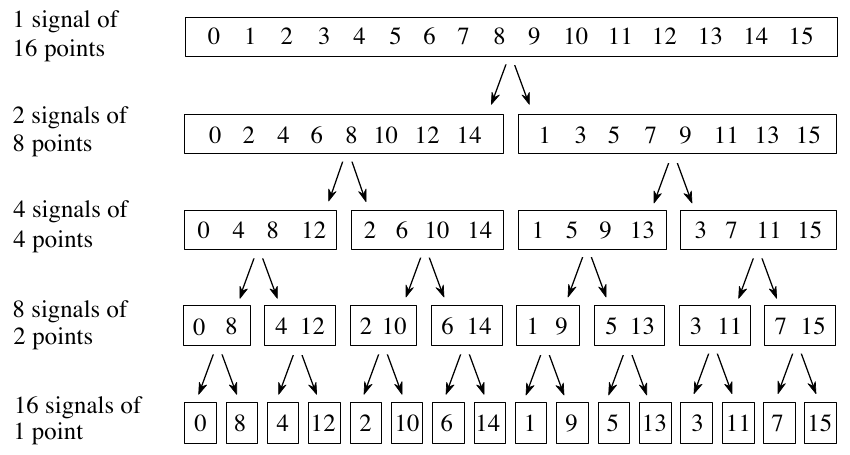
\includegraphics[width=0.708\linewidth,height=0.8\textheight,keepaspectratio]{assets/ch12/fig12-02.png}
\caption*{\textbf{图 12-2　FFT 的分解。} 一个 N 点信号被分解成 N
个各含一个点的信号。每个阶段都使用交错分解，把偶数号和奇数号采样分开。
（左侧从上到下：1 signal of 16 points = 1 个 16 点信号，2 signals of 8
points = 2 个 8 点信号，4 signals of 4 points = 4 个 4 点信号，8 signals
of 2 points = 8 个 2 点信号，16 signals of 1 point = 16 个 1 点信号。）}
\end{figure}

明白了分解的结构，就可以大大简化它。这种分解不过是把信号中的采样重新排序。图
12-3
给出了所需的重排规律。左边列出原信号的采样序号及其二进制形式；右边列出重排后的采样序号，也附上二进制形式。关键在于：左右两边的二进制数互为位反转。例如，第
3 个采样（0011）与第 12 个采样（1100）交换；同样，第 14
个采样（1110）与第 7 个采样（0111）交换，依此类推。FFT
的时域分解通常用位反转排序(bit reversal
sorting)算法完成，也就是把二进制数的位左右颠倒后计数，按这个顺序重排 N
个时域采样（就像图 12-3 最右一列那样）。

\begin{figure}[htbp]
\centering
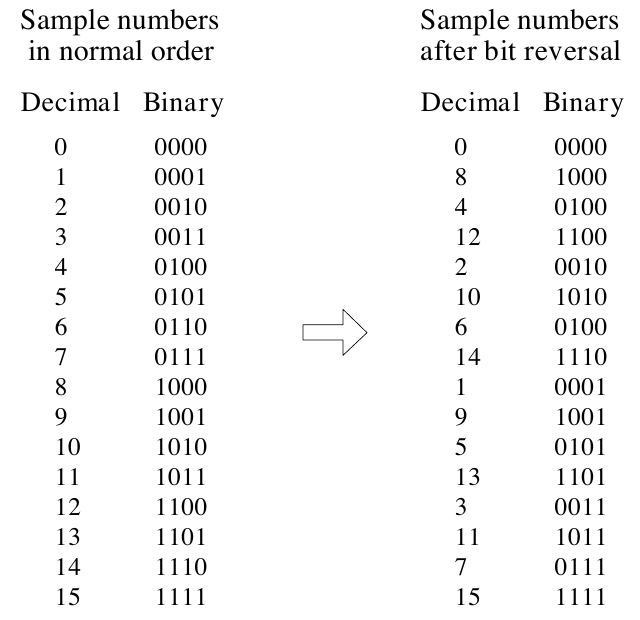
\includegraphics[width=0.533\linewidth,height=0.8\textheight,keepaspectratio]{assets/ch12/fig12-03.png}
\caption*{\textbf{图 12-3　FFT 的位反转排序。} FFT
的时域分解可以通过按位反转顺序给采样排序来实现。 （Sample numbers in
normal order = 正常顺序的采样序号，Sample numbers after bit reversal =
位反转后的采样序号；Decimal = 十进制，Binary = 二进制。原图右栏第 7
行十进制 6 的二进制印成了 0100，应为 0110。）}
\end{figure}

FFT 算法的下一步，是求这些 1 点时域信号的频谱。这再简单不过了：1
点信号的频谱就等于它自己。这意味着这一步什么都不用做。虽然不用做任何工作，别忘了：现在每个
1 点信号都是一个频谱，而不再是时域信号了。

FFT 的最后一步，是按与时域分解完全相反的顺序，把这 N
个频谱合并起来。算法从这里开始变得麻烦。可惜位反转这条捷径在这里用不上，我们必须一次退回一个阶段。在第一阶段，16
个频谱（每个 1 点）合成 8 个频谱（每个 2 点）。在第二阶段，8
个频谱（每个 2 点）合成 4 个频谱（每个 4
点），依此类推。最后一个阶段产生 FFT 的输出：一个 16 点频谱。

图 12-4 展示了两个各含 4 点的频谱怎样合并成一个 8
点频谱。这种合成必须撤销时域中所做的交错分解。换句话说，频域中的操作必须对应时域中''把两个
4 点信号交错合并''的过程。考虑两个时域信号 abcd 和
efgh。可以分两步得到一个 8 点时域信号：先在每个 4
点信号中插入零，把它稀释(dilute)成 8
点信号，然后把两个信号相加。也就是说，abcd 变成 a0b0c0d0，efgh 变成
0e0f0g0h，这两个 8 点信号相加得到 aebfcgdh。如图 12-4
所示，在时域中插零稀释，对应频谱的复制。因此，FFT
中合并频谱的方法，就是把它们复制一遍，再把复制后的频谱相加。

\begin{figure}[htbp]
\centering
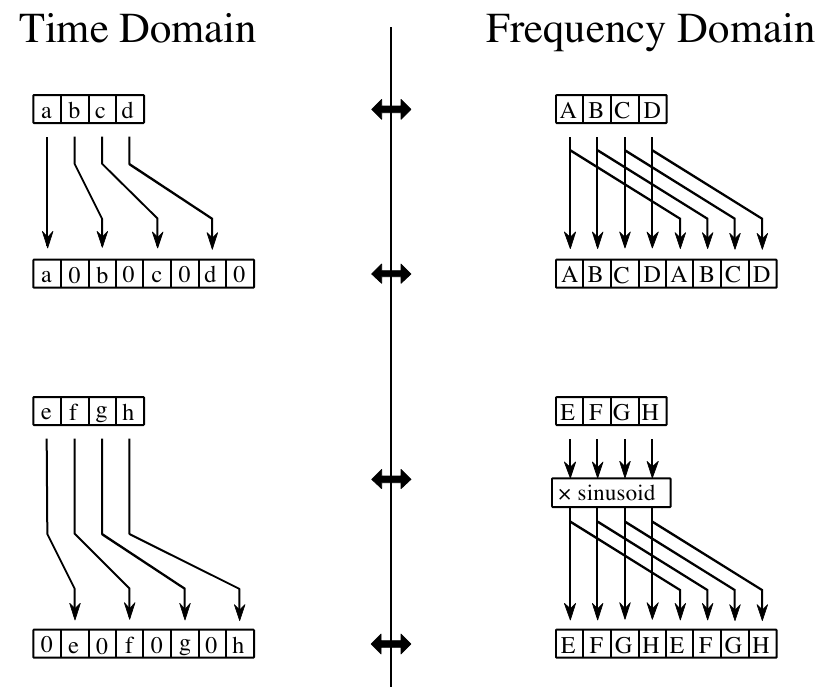
\includegraphics[width=0.692\linewidth,height=0.8\textheight,keepaspectratio]{assets/ch12/fig12-04.png}
\caption*{\textbf{图 12-4　FFT 的合成。}
时域信号插零稀释时，频域被复制一遍。如果稀释时时域信号还平移了一个采样，频谱还要再乘上一个正弦曲线。
（Time Domain = 时域，Frequency Domain = 频域，× sinusoid =
乘以正弦曲线。）}
\end{figure}

为了相加时能对上，两个时域信号的插零方式略有不同：一个信号的奇数点为零，另一个信号的偶数点为零。换句话说，其中一个时域信号（图
12-4 中的
0e0f0g0h）向右平移了一个采样。时域的这个平移，对应频谱乘上一个正弦曲线(sinusoid)。要看清这一点，回忆一下：时域中的平移等价于把信号与一个平移过的冲激函数卷积，这相当于把信号的频谱乘以平移冲激函数的频谱，而平移冲激函数的频谱是一条正弦曲线（见图
11-2）。

\begin{figure}[htbp]
\centering
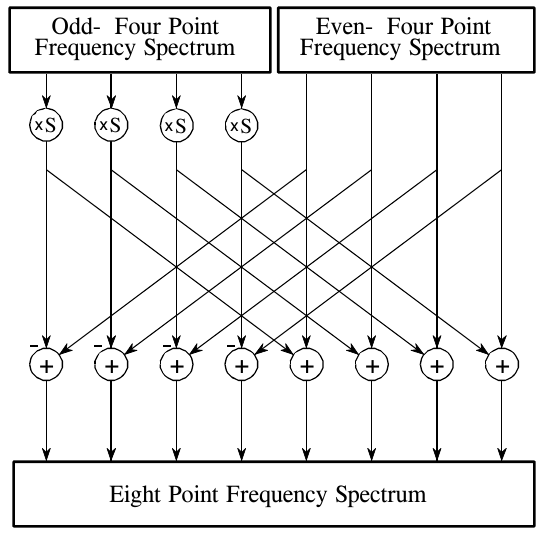
\includegraphics[width=0.458\linewidth,height=0.8\textheight,keepaspectratio]{assets/ch12/fig12-05.png}
\caption*{\textbf{图 12-5　FFT 合成流程图。} 这里展示了把两个 4 点频谱合并成一个 8
点频谱的方法。×S 运算表示把信号乘以一个频率选取得当的正弦曲线。 （Odd-
Four Point Frequency Spectrum = 奇数点的 4 点频谱，Even- Four Point
Frequency Spectrum = 偶数点的 4 点频谱，Eight Point Frequency Spectrum =
8 点频谱；加号旁的 − 表示该路相减。）}
\end{figure}

图 12-5 是把两个 4 点频谱合并成一个 8
点频谱的流程图。再进一步简化：注意图 12-5 是由图 12-6
中的基本模式一再重复构成的。这个简单的流程图因为形似翅膀而被称为蝶形(butterfly)。蝶形是
FFT 的基本计算单元，它把两个复数点变换成另外两个复数点。

\begin{figure}[htbp]
\centering
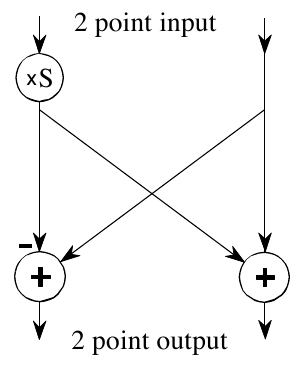
\includegraphics[width=0.254\linewidth,height=0.8\textheight,keepaspectratio]{assets/ch12/fig12-06.png}
\caption*{\textbf{图 12-6　FFT 蝶形。} 这是 FFT
的基本计算单元，取两个复数点，把它们变换成另外两个复数点。 （2 point
input = 2 点输入，2 point output = 2 点输出，×S = 乘以正弦曲线。）}
\end{figure}

图 12-7 展示了整个 FFT
的结构。时域分解由位反转排序算法完成。把分解后的数据变换到频域不需要做任何事，所以图中没有出现这一步。

频域合成需要三重循环。外层循环遍历 \(\log_2 N\) 个阶段（即图 12-2
中的每一层，从下往上）。中层循环遍历当前阶段中的每个频谱（即图 12-2
中任意一层上的每个方框）。最内层循环用蝶形计算每个频谱中的各个点（即遍历图
12-2 中任意一个方框里的采样）。图 12-7
中的''开销''(overhead)方框负责确定循环的起止下标，并计算蝶形所需的正弦曲线。现在我们来到本章的核心：实际的
FFT 程序。

\begin{figure}[htbp]
\centering
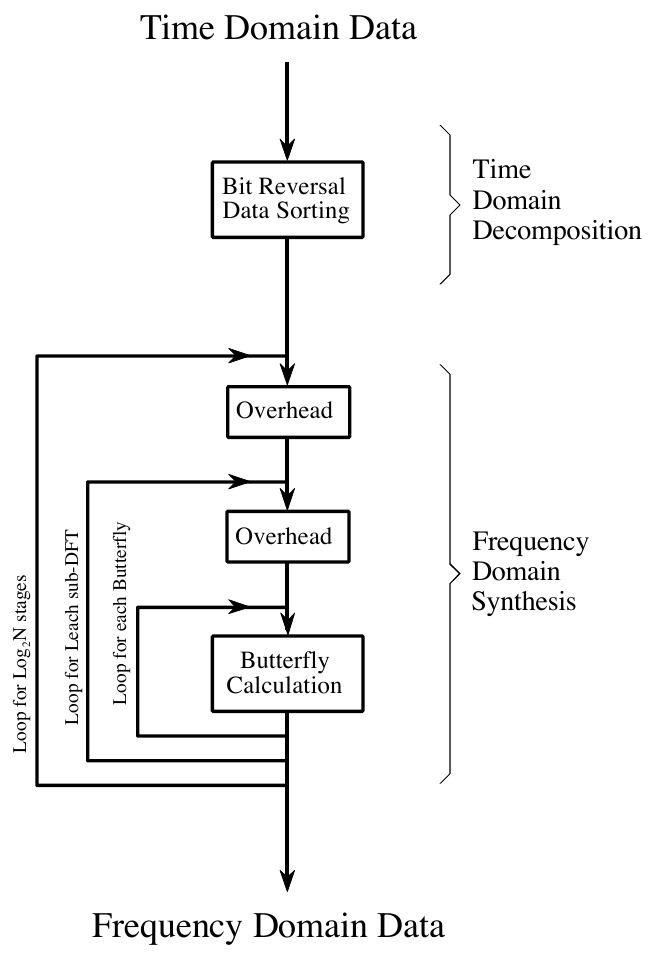
\includegraphics[width=0.546\linewidth,height=0.8\textheight,keepaspectratio]{assets/ch12/fig12-07.png}
\caption*{\textbf{图 12-7　FFT 流程图。} 它基于三个步骤：(1) 把一个 N
点时域信号分解成 N 个各含一个点的信号；(2) 求这 N
个点信号各自的频谱（什么都不用做）；(3) 把这 N 个频谱合成为一个频谱。
（Time Domain Data = 时域数据，Bit Reversal Data Sorting =
位反转数据排序，Time Domain Decomposition = 时域分解；Overhead =
开销（准备循环下标和正弦值），Butterfly Calculation =
蝶形计算，Frequency Domain Synthesis = 频域合成，Frequency Domain Data =
频域数据。三个循环从外到内：Loop for Log₂N stages = 遍历 log₂N
个阶段，Loop for each sub-DFT = 遍历每个子 DFT（原图误印为 Leach），Loop
for each Butterfly = 遍历每个蝶形。）}
\end{figure}

\section{FFT 程序}

第 8 章讲过，实数 DFT
可以通过把时域信号与正弦波和余弦波做相关来计算（见表 8-2）。表 12-2
给出了用同样的方法计算复数 DFT 的程序。公平对比的话，FFT
改进的正是这个程序。

\textbf{表 12-2}（注释已译成中文）

\begin{Shaded}
\begin{Highlighting}[]
\NormalTok{5000 \textquotesingle{}COMPLEX DFT BY CORRELATION}
\NormalTok{5010 \textquotesingle{}进入时，N\% 是 DFT 的点数，}
\NormalTok{5020 \textquotesingle{}XR[ ] 和 XI[ ] 是时域的实部和虚部。}
\NormalTok{5030 \textquotesingle{}返回时，REX[ ] 和 IMX[ ] 存放频域数据。}
\NormalTok{5040 \textquotesingle{}所有信号都从 0 到 N\%{-}1。}
\NormalTok{5050 \textquotesingle{}}
\NormalTok{5060 PI = 3.14159265                           \textquotesingle{}设置常数}
\NormalTok{5070 \textquotesingle{}}
\NormalTok{5080 FOR K\% = 0 TO N\%{-}1                        \textquotesingle{}把 REX[ ] 和 IMX[ ] 清零，}
\NormalTok{5090 REX[K\%] = 0                               \textquotesingle{}以便相关时当累加器用}
\NormalTok{5100 IMX[K\%] = 0}
\NormalTok{5110 NEXT K\%}
\NormalTok{5120 \textquotesingle{}}
\NormalTok{5130 FOR K\% = 0 TO N\%{-}1                        \textquotesingle{}遍历频域的每个值}
\NormalTok{5140 FOR I\% = 0 TO N\%{-}1                        \textquotesingle{}与复正弦 SR 和 SI 做相关}
\NormalTok{5150 \textquotesingle{}}
\NormalTok{5160 SR = COS(2*PI*K\%*I\%/N\%)                   \textquotesingle{}计算复正弦}
\NormalTok{5170 SI = {-}SIN(2*PI*K\%*I\%/N\%)}
\NormalTok{5180 REX[K\%] = REX[K\%] + XR[I\%]*SR {-} XI[I\%]*SI}
\NormalTok{5190 IMX[K\%] = IMX[K\%] + XR[I\%]*SI + XI[I\%]*SR}
\NormalTok{5200 \textquotesingle{}}
\NormalTok{5210 NEXT I\%}
\NormalTok{5220 NEXT K\%}
\NormalTok{5230 \textquotesingle{}}
\NormalTok{5240 RETURN}
\end{Highlighting}
\end{Shaded}

\textbf{C 实现}（完整可编译版本见
\texttt{c/table12-2\_complex\_dft\_correlation.c}）：

\begin{Shaded}
\begin{Highlighting}[]
\CommentTok{/* 5000：相关法复数 DFT。xr/xi 是时域，rex/imx 是频域，下标都是 0～n{-}1 */}
\DataTypeTok{static} \DataTypeTok{void}\NormalTok{ complex\_dft}\OperatorTok{(}\DataTypeTok{const} \DataTypeTok{double} \OperatorTok{*}\NormalTok{xr}\OperatorTok{,} \DataTypeTok{const} \DataTypeTok{double} \OperatorTok{*}\NormalTok{xi}\OperatorTok{,} \DataTypeTok{int}\NormalTok{ n}\OperatorTok{,} \DataTypeTok{double} \OperatorTok{*}\NormalTok{rex}\OperatorTok{,} \DataTypeTok{double} \OperatorTok{*}\NormalTok{imx}\OperatorTok{)}
\OperatorTok{\{}
    \ControlFlowTok{for} \OperatorTok{(}\DataTypeTok{int}\NormalTok{ k }\OperatorTok{=} \DecValTok{0}\OperatorTok{;}\NormalTok{ k }\OperatorTok{\textless{}}\NormalTok{ n}\OperatorTok{;}\NormalTok{ k}\OperatorTok{++)} \OperatorTok{\{}           \CommentTok{/* 5080～5110：REX[]、IMX[] 清零，相关时当累加器用 */}
\NormalTok{        rex}\OperatorTok{[}\NormalTok{k}\OperatorTok{]} \OperatorTok{=} \FloatTok{0.0}\OperatorTok{;}
\NormalTok{        imx}\OperatorTok{[}\NormalTok{k}\OperatorTok{]} \OperatorTok{=} \FloatTok{0.0}\OperatorTok{;}
    \OperatorTok{\}}
    \ControlFlowTok{for} \OperatorTok{(}\DataTypeTok{int}\NormalTok{ k }\OperatorTok{=} \DecValTok{0}\OperatorTok{;}\NormalTok{ k }\OperatorTok{\textless{}}\NormalTok{ n}\OperatorTok{;}\NormalTok{ k}\OperatorTok{++)}             \CommentTok{/* 5130：遍历频域的每个点 */}
        \ControlFlowTok{for} \OperatorTok{(}\DataTypeTok{int}\NormalTok{ i }\OperatorTok{=} \DecValTok{0}\OperatorTok{;}\NormalTok{ i }\OperatorTok{\textless{}}\NormalTok{ n}\OperatorTok{;}\NormalTok{ i}\OperatorTok{++)} \OperatorTok{\{}       \CommentTok{/* 5140：与复正弦 SR、SI 做相关 */}
            \DataTypeTok{double}\NormalTok{ sr }\OperatorTok{=}\NormalTok{ cos}\OperatorTok{(}\FloatTok{2.0} \OperatorTok{*}\NormalTok{ PI }\OperatorTok{*}\NormalTok{ k }\OperatorTok{*}\NormalTok{ i }\OperatorTok{/}\NormalTok{ n}\OperatorTok{);}      \CommentTok{/* 5160～5170：算出复正弦 */}
            \DataTypeTok{double}\NormalTok{ si }\OperatorTok{=} \OperatorTok{{-}}\NormalTok{sin}\OperatorTok{(}\FloatTok{2.0} \OperatorTok{*}\NormalTok{ PI }\OperatorTok{*}\NormalTok{ k }\OperatorTok{*}\NormalTok{ i }\OperatorTok{/}\NormalTok{ n}\OperatorTok{);}
\NormalTok{            rex}\OperatorTok{[}\NormalTok{k}\OperatorTok{]} \OperatorTok{+=}\NormalTok{ xr}\OperatorTok{[}\NormalTok{i}\OperatorTok{]} \OperatorTok{*}\NormalTok{ sr }\OperatorTok{{-}}\NormalTok{ xi}\OperatorTok{[}\NormalTok{i}\OperatorTok{]} \OperatorTok{*}\NormalTok{ si}\OperatorTok{;}          \CommentTok{/* 5180～5190：复数乘法后累加 */}
\NormalTok{            imx}\OperatorTok{[}\NormalTok{k}\OperatorTok{]} \OperatorTok{+=}\NormalTok{ xr}\OperatorTok{[}\NormalTok{i}\OperatorTok{]} \OperatorTok{*}\NormalTok{ si }\OperatorTok{+}\NormalTok{ xi}\OperatorTok{[}\NormalTok{i}\OperatorTok{]} \OperatorTok{*}\NormalTok{ sr}\OperatorTok{;}
        \OperatorTok{\}}
\OperatorTok{\}}
\end{Highlighting}
\end{Shaded}

运行结果（N=64）：冲激的频谱处处为 1+0j（偏差为 0）；频率为 5
的复正弦只在 X{[}5{]} 处得到 64，其余点幅度不超过
1.1e-13；实信号的频谱满足''实部偶对称、虚部奇对称''，偏差 1.0e-13。

表 12-3 和表 12-4 是两个不同的 FFT 程序，一个用 FORTRAN 写，一个用 BASIC
写。先看表 12-4 的 BASIC 子程序。它产生的输出与表 12-2
的相关法完全相同，只是快得多。可以用图 12-7
的方框图来辨认这个程序的各个部分。数据通过数组 REX{[} {]} 和 IMX{[} {]}
传给这个 FFT 子程序，下标都从 0 到 N−1。从子程序返回时，REX{[} {]} 和
IMX{[} {]} 被频域数据覆盖。这是 FFT
高度优化的又一个体现：输入、中间存储和输出都用同一组数组。这种高效的内存使用，对设计计算
FFT 的高速硬件很重要。描述这种内存用法的术语叫原地计算(in-place
computation)。

所有 FFT 程序得到的数值结果都一样，但在编程上有些细微差别需要留意。表
12-3 的 FORTRAN
程序体现了其中几种差别。这个程序使用一种叫按频率抽取(decimation in
frequency)的算法，而前面介绍的算法叫按时间抽取(decimation in
time)。在按频率抽取的算法中，位反转排序放在三重嵌套循环之后进行。还有一些
FFT 程序完全省掉了位反转排序。这些变体都不能显著提高 FFT
的性能，你不必操心用的是哪一种。

FFT 算法之间重要的差别，在于数据怎样传入和传出子程序。在 BASIC
程序中，数据通过数组 REX{[} {]} 和 IMX{[} {]} 进出子程序，采样下标从 0
到 N−1。在 FORTRAN 程序中，数据通过复数数组 X( ) 传递，采样下标从 1 到
N。由于这是一个复数变量数组，X( )
中的每个采样都由两个数组成：实部和虚部。DFT
的长度也必须传给这些子程序。BASIC 程序用变量 N\% 来传；相比之下，FORTRAN
程序用变量 M，它定义为 \(\log_2 N\)。例如，256 点 DFT 的 M 是 8，4096 点
DFT 的 M 是 12，等等。要点是，写 FFT
子程序的程序员在怎样与主程序对接方面有很多选择。像 FORTRAN 程序这样从 1
到 N 的数组尤其让人恼火。大多数 DSP 文献（包括本书）都假定数组从第 0
到第 N−1 个采样来讲解算法。例如，如果数组从 1 到 N，频域的对称中心就是第
1 点和第 N/2+1 点，而不是第 0 点和第 N/2 点。

\textbf{表 12-3　用 FORTRAN 写的快速傅里叶变换。} 数据通过变量 X( ) 和 M
传给这个子程序。整数 M 是 DFT 长度的以 2 为底的对数，例如 256 点 DFT 的
M = 8，4096 点 DFT 的 M = 12，等等。复数数组 X( )
在进入时存放时域数据，从子程序返回时被频域数据覆盖。注意：这个子程序要求输入和输出信号从
X(1) 到 X(N)，而不是通常的 X(0) 到 X(N−1)。

\begin{Shaded}
\begin{Highlighting}[]
      \KeywordTok{SUBROUTINE}\NormalTok{ FFT(X,M)}
      \DataTypeTok{COMPLEX}\NormalTok{ X(}\DecValTok{4096}\NormalTok{),U,S,T}
\NormalTok{      PI}\KeywordTok{=}\FloatTok{3.14159265}
\NormalTok{      N}\KeywordTok{=}\DecValTok{2}\KeywordTok{**}\NormalTok{M}
      \KeywordTok{DO} \DecValTok{20}\NormalTok{ L}\KeywordTok{=}\DecValTok{1}\NormalTok{,M}
\NormalTok{      LE}\KeywordTok{=}\DecValTok{2}\KeywordTok{**}\NormalTok{(M}\KeywordTok{+}\DecValTok{1}\KeywordTok{{-}}\NormalTok{L)}
\NormalTok{      LE2}\KeywordTok{=}\NormalTok{LE}\KeywordTok{/}\DecValTok{2}
\NormalTok{      U}\KeywordTok{=}\NormalTok{(}\FloatTok{1.0}\NormalTok{,}\FloatTok{0.0}\NormalTok{)}
\NormalTok{      S}\KeywordTok{=}\BuiltInTok{CMPLX}\NormalTok{(}\BuiltInTok{COS}\NormalTok{(PI}\KeywordTok{/}\BuiltInTok{FLOAT}\NormalTok{(LE2)),}\KeywordTok{{-}}\BuiltInTok{SIN}\NormalTok{(PI}\KeywordTok{/}\BuiltInTok{FLOAT}\NormalTok{(LE2)))}
      \KeywordTok{DO} \DecValTok{20}\NormalTok{ J}\KeywordTok{=}\DecValTok{1}\NormalTok{,LE2}
      \KeywordTok{DO} \DecValTok{10}\NormalTok{ I}\KeywordTok{=}\NormalTok{J,N,LE}
\NormalTok{      IP}\KeywordTok{=}\NormalTok{I}\KeywordTok{+}\NormalTok{LE2}
\NormalTok{      T}\KeywordTok{=}\NormalTok{X(I)}\KeywordTok{+}\NormalTok{X(IP)}
\NormalTok{      X(IP)}\KeywordTok{=}\NormalTok{(X(I)}\KeywordTok{{-}}\NormalTok{X(IP))}\KeywordTok{*}\NormalTok{U}
 \DecValTok{10}\NormalTok{   X(I)}\KeywordTok{=}\NormalTok{T}
 \DecValTok{20}\NormalTok{   U}\KeywordTok{=}\NormalTok{U}\KeywordTok{*}\NormalTok{S}
\NormalTok{      ND2}\KeywordTok{=}\NormalTok{N}\KeywordTok{/}\DecValTok{2}
\NormalTok{      NM1}\KeywordTok{=}\NormalTok{N}\KeywordTok{{-}}\DecValTok{1}
\NormalTok{      J}\KeywordTok{=}\DecValTok{1}
      \KeywordTok{DO} \DecValTok{50}\NormalTok{ I}\KeywordTok{=}\DecValTok{1}\NormalTok{,NM1}
      \KeywordTok{IF}\NormalTok{(I}\OperatorTok{.GE.}\NormalTok{J) }\KeywordTok{GO} \KeywordTok{TO} \DecValTok{30}
\NormalTok{      T}\KeywordTok{=}\NormalTok{X(J)}
\NormalTok{      X(J)}\KeywordTok{=}\NormalTok{X(I)}
\NormalTok{      X(I)}\KeywordTok{=}\NormalTok{T}
 \DecValTok{30}\NormalTok{   K}\KeywordTok{=}\NormalTok{ND2}
 \DecValTok{40}   \KeywordTok{IF}\NormalTok{(K}\OperatorTok{.GE.}\NormalTok{J) }\KeywordTok{GO} \KeywordTok{TO} \DecValTok{50}
\NormalTok{      J}\KeywordTok{=}\NormalTok{J}\KeywordTok{{-}}\NormalTok{K}
\NormalTok{      K}\KeywordTok{=}\NormalTok{K}\KeywordTok{/}\DecValTok{2}
      \KeywordTok{GO} \KeywordTok{TO} \DecValTok{40}
 \DecValTok{50}\NormalTok{   J}\KeywordTok{=}\NormalTok{J}\KeywordTok{+}\NormalTok{K}
      \KeywordTok{RETURN}
      \KeywordTok{END}
\end{Highlighting}
\end{Shaded}

\textbf{C 实现}（完整可编译版本见
\texttt{c/table12-3\_fft\_fortran.c}。为了逐行对照，C 版本同样用从 1
开始的下标，复数用 C99 的 \texttt{double\ complex}）：

\begin{Shaded}
\begin{Highlighting}[]
\CommentTok{/* SUBROUTINE FFT(X,M)：x[1]～x[n] 进为时域、出为频域 */}
\DataTypeTok{static} \DataTypeTok{void}\NormalTok{ fft\_fortran}\OperatorTok{(}\DataTypeTok{double} \DataTypeTok{complex} \OperatorTok{*}\NormalTok{x}\OperatorTok{,} \DataTypeTok{int}\NormalTok{ m}\OperatorTok{)}
\OperatorTok{\{}
    \DataTypeTok{int}\NormalTok{ n }\OperatorTok{=} \DecValTok{1} \OperatorTok{\textless{}\textless{}}\NormalTok{ m}\OperatorTok{;}                                         \CommentTok{/* N=2**M */}
    \ControlFlowTok{for} \OperatorTok{(}\DataTypeTok{int}\NormalTok{ l }\OperatorTok{=} \DecValTok{1}\OperatorTok{;}\NormalTok{ l }\OperatorTok{\textless{}=}\NormalTok{ m}\OperatorTok{;}\NormalTok{ l}\OperatorTok{++)} \OperatorTok{\{}                          \CommentTok{/* DO 20 L=1,M：遍历每一级 */}
        \DataTypeTok{int}\NormalTok{ le }\OperatorTok{=} \DecValTok{1} \OperatorTok{\textless{}\textless{}} \OperatorTok{(}\NormalTok{m }\OperatorTok{+} \DecValTok{1} \OperatorTok{{-}}\NormalTok{ l}\OperatorTok{);}                          \CommentTok{/* LE=2**(M+1{-}L)：本级子 DFT 的长度，从 N 开始逐级减半 */}
        \DataTypeTok{int}\NormalTok{ le2 }\OperatorTok{=}\NormalTok{ le }\OperatorTok{/} \DecValTok{2}\OperatorTok{;}
        \DataTypeTok{double} \DataTypeTok{complex}\NormalTok{ u }\OperatorTok{=} \FloatTok{1.0}\OperatorTok{;}                             \CommentTok{/* U=(1.0,0.0) */}
        \DataTypeTok{double} \DataTypeTok{complex}\NormalTok{ s }\OperatorTok{=}\NormalTok{ cos}\OperatorTok{(}\NormalTok{PI }\OperatorTok{/}\NormalTok{ le2}\OperatorTok{)} \OperatorTok{{-}}\NormalTok{ I }\OperatorTok{*}\NormalTok{ sin}\OperatorTok{(}\NormalTok{PI }\OperatorTok{/}\NormalTok{ le2}\OperatorTok{);}   \CommentTok{/* S=CMPLX(COS(PI/LE2),{-}SIN(PI/LE2)) */}
        \ControlFlowTok{for} \OperatorTok{(}\DataTypeTok{int}\NormalTok{ j }\OperatorTok{=} \DecValTok{1}\OperatorTok{;}\NormalTok{ j }\OperatorTok{\textless{}=}\NormalTok{ le2}\OperatorTok{;}\NormalTok{ j}\OperatorTok{++)} \OperatorTok{\{}                    \CommentTok{/* DO 20 J=1,LE2 */}
            \ControlFlowTok{for} \OperatorTok{(}\DataTypeTok{int}\NormalTok{ i }\OperatorTok{=}\NormalTok{ j}\OperatorTok{;}\NormalTok{ i }\OperatorTok{\textless{}=}\NormalTok{ n}\OperatorTok{;}\NormalTok{ i }\OperatorTok{+=}\NormalTok{ le}\OperatorTok{)} \OperatorTok{\{}              \CommentTok{/* DO 10 I=J,N,LE：遍历每个蝶形 */}
                \DataTypeTok{int}\NormalTok{ ip }\OperatorTok{=}\NormalTok{ i }\OperatorTok{+}\NormalTok{ le2}\OperatorTok{;}
                \DataTypeTok{double} \DataTypeTok{complex}\NormalTok{ t }\OperatorTok{=}\NormalTok{ x}\OperatorTok{[}\NormalTok{i}\OperatorTok{]} \OperatorTok{+}\NormalTok{ x}\OperatorTok{[}\NormalTok{ip}\OperatorTok{];}            \CommentTok{/* T=X(I)+X(IP) */}
\NormalTok{                x}\OperatorTok{[}\NormalTok{ip}\OperatorTok{]} \OperatorTok{=} \OperatorTok{(}\NormalTok{x}\OperatorTok{[}\NormalTok{i}\OperatorTok{]} \OperatorTok{{-}}\NormalTok{ x}\OperatorTok{[}\NormalTok{ip}\OperatorTok{])} \OperatorTok{*}\NormalTok{ u}\OperatorTok{;}                 \CommentTok{/* X(IP)=(X(I){-}X(IP))*U：先相减再乘正弦，与按时间抽取的蝶形相反 */}
\NormalTok{                x}\OperatorTok{[}\NormalTok{i}\OperatorTok{]} \OperatorTok{=}\NormalTok{ t}\OperatorTok{;}                                   \CommentTok{/* 10 X(I)=T */}
            \OperatorTok{\}}
\NormalTok{            u }\OperatorTok{=}\NormalTok{ u }\OperatorTok{*}\NormalTok{ s}\OperatorTok{;}                                      \CommentTok{/* 20 U=U*S：标号 20 属于 J 循环，每个 J 转一次 */}
        \OperatorTok{\}}
    \OperatorTok{\}}

    \DataTypeTok{int}\NormalTok{ nd2 }\OperatorTok{=}\NormalTok{ n }\OperatorTok{/} \DecValTok{2}\OperatorTok{,}\NormalTok{ nm1 }\OperatorTok{=}\NormalTok{ n }\OperatorTok{{-}} \DecValTok{1}\OperatorTok{,}\NormalTok{ j }\OperatorTok{=} \DecValTok{1}\OperatorTok{;}                    \CommentTok{/* ND2=N/2，NM1=N{-}1，J=1 */}
    \ControlFlowTok{for} \OperatorTok{(}\DataTypeTok{int}\NormalTok{ i }\OperatorTok{=} \DecValTok{1}\OperatorTok{;}\NormalTok{ i }\OperatorTok{\textless{}=}\NormalTok{ nm1}\OperatorTok{;}\NormalTok{ i}\OperatorTok{++)} \OperatorTok{\{}                        \CommentTok{/* DO 50 I=1,NM1：位反转排序 */}
        \ControlFlowTok{if} \OperatorTok{(}\NormalTok{i }\OperatorTok{\textless{}}\NormalTok{ j}\OperatorTok{)} \OperatorTok{\{}                                        \CommentTok{/* IF(I.GE.J) GO TO 30 */}
            \DataTypeTok{double} \DataTypeTok{complex}\NormalTok{ t }\OperatorTok{=}\NormalTok{ x}\OperatorTok{[}\NormalTok{j}\OperatorTok{];}
\NormalTok{            x}\OperatorTok{[}\NormalTok{j}\OperatorTok{]} \OperatorTok{=}\NormalTok{ x}\OperatorTok{[}\NormalTok{i}\OperatorTok{];}
\NormalTok{            x}\OperatorTok{[}\NormalTok{i}\OperatorTok{]} \OperatorTok{=}\NormalTok{ t}\OperatorTok{;}
        \OperatorTok{\}}
        \DataTypeTok{int}\NormalTok{ k }\OperatorTok{=}\NormalTok{ nd2}\OperatorTok{;}                                        \CommentTok{/* 30 K=ND2 */}
        \ControlFlowTok{while} \OperatorTok{(}\NormalTok{k }\OperatorTok{\textless{}}\NormalTok{ j}\OperatorTok{)} \OperatorTok{\{}                                     \CommentTok{/* 40 IF(K.GE.J) GO TO 50 */}
\NormalTok{            j }\OperatorTok{{-}=}\NormalTok{ k}\OperatorTok{;}                                         \CommentTok{/* J=J{-}K */}
\NormalTok{            k }\OperatorTok{/=} \DecValTok{2}\OperatorTok{;}                                         \CommentTok{/* K=K/2，GO TO 40 */}
        \OperatorTok{\}}
\NormalTok{        j }\OperatorTok{+=}\NormalTok{ k}\OperatorTok{;}                                             \CommentTok{/* 50 J=J+K */}
    \OperatorTok{\}}
\OperatorTok{\}}
\end{Highlighting}
\end{Shaded}

运行结果：随机复信号与相关法复数 DFT 逐点比较，最大偏差 N=8 时
1.9e-15，N=64 时 1.4e-13，N=1024 时 1.0e-11。

\textbf{表 12-4　用 BASIC 写的快速傅里叶变换。}（注释已译成中文）

\begin{Shaded}
\begin{Highlighting}[]
\NormalTok{1000 \textquotesingle{}THE FAST FOURIER TRANSFORM}
\NormalTok{1010 \textquotesingle{}进入时，N\% 是 DFT 的点数，REX[ ] 和}
\NormalTok{1020 \textquotesingle{}IMX[ ] 是输入的实部和虚部。返回时，}
\NormalTok{1030 \textquotesingle{}REX[ ] 和 IMX[ ] 存放 DFT 的输出。所有信号都从 0 到 N\%{-}1。}
\NormalTok{1040 \textquotesingle{}}
\NormalTok{1050 PI = 3.14159265                                    \textquotesingle{}设置常数}
\NormalTok{1060 NM1\% = N\%{-}1}
\NormalTok{1070 ND2\% = N\%/2}
\NormalTok{1080 M\% = CINT(LOG(N\%)/LOG(2))}
\NormalTok{1090 J\% = ND2\%}
\NormalTok{1100 \textquotesingle{}}
\NormalTok{1110 FOR I\% = 1 TO N\%{-}2                                 \textquotesingle{}位反转排序}
\NormalTok{1120 IF I\% \textgreater{}= J\% THEN GOTO 1190}
\NormalTok{1130 TR = REX[J\%]}
\NormalTok{1140 TI = IMX[J\%]}
\NormalTok{1150 REX[J\%] = REX[I\%]}
\NormalTok{1160 IMX[J\%] = IMX[I\%]}
\NormalTok{1170 REX[I\%] = TR}
\NormalTok{1180 IMX[I\%] = TI}
\NormalTok{1190 K\% = ND2\%}
\NormalTok{1200 IF K\% \textgreater{} J\% THEN GOTO 1240}
\NormalTok{1210 J\% = J\%{-}K\%}
\NormalTok{1220 K\% = K\%/2}
\NormalTok{1230 GOTO 1200}
\NormalTok{1240 J\% = J\%+K\%}
\NormalTok{1250 NEXT I\%}
\NormalTok{1260 \textquotesingle{}}
\NormalTok{1270 FOR L\% = 1 TO M\%                                   \textquotesingle{}遍历每一级}
\NormalTok{1280 LE\% = CINT(2\^{}L\%)}
\NormalTok{1290 LE2\% = LE\%/2}
\NormalTok{1300 UR = 1}
\NormalTok{1310 UI = 0}
\NormalTok{1320 SR = COS(PI/LE2\%)                                  \textquotesingle{}计算正弦和余弦值}
\NormalTok{1330 SI = {-}SIN(PI/LE2\%)}
\NormalTok{1340 FOR J\% = 1 TO LE2\%                                 \textquotesingle{}遍历每个子 DFT}
\NormalTok{1350 JM1\% = J\%{-}1}
\NormalTok{1360 FOR I\% = JM1\% TO NM1\% STEP LE\%                     \textquotesingle{}遍历每个蝶形}
\NormalTok{1370     IP\% = I\%+LE2\%}
\NormalTok{1380     TR = REX[IP\%]*UR {-} IMX[IP\%]*UI                 \textquotesingle{}蝶形计算}
\NormalTok{1390     TI = REX[IP\%]*UI + IMX[IP\%]*UR}
\NormalTok{1400     REX[IP\%] = REX[I\%]{-}TR}
\NormalTok{1410     IMX[IP\%] = IMX[I\%]{-}TI}
\NormalTok{1420     REX[I\%] = REX[I\%]+TR}
\NormalTok{1430     IMX[I\%] = IMX[I\%]+TI}
\NormalTok{1440 NEXT I\%}
\NormalTok{1450 TR = UR}
\NormalTok{1460 UR = TR*SR {-} UI*SI}
\NormalTok{1470 UI = TR*SI + UI*SR}
\NormalTok{1480 NEXT J\%}
\NormalTok{1490 NEXT L\%}
\NormalTok{1500 \textquotesingle{}}
\NormalTok{1510 RETURN}
\end{Highlighting}
\end{Shaded}

\textbf{C 实现}（完整可编译版本见 \texttt{c/table12-4\_fft.c}）：

\begin{Shaded}
\begin{Highlighting}[]
\CommentTok{/* 1110～1250：位反转排序 */}
\DataTypeTok{static} \DataTypeTok{void}\NormalTok{ bit\_reversal\_sort}\OperatorTok{(}\DataTypeTok{double} \OperatorTok{*}\NormalTok{rex}\OperatorTok{,} \DataTypeTok{double} \OperatorTok{*}\NormalTok{imx}\OperatorTok{,} \DataTypeTok{int}\NormalTok{ n}\OperatorTok{)}
\OperatorTok{\{}
    \DataTypeTok{int}\NormalTok{ nd2 }\OperatorTok{=}\NormalTok{ n }\OperatorTok{/} \DecValTok{2}\OperatorTok{,}\NormalTok{ j }\OperatorTok{=}\NormalTok{ nd2}\OperatorTok{;}                   \CommentTok{/* 1070、1090：ND2\% = N\%/2，J\% = ND2\% */}
    \ControlFlowTok{for} \OperatorTok{(}\DataTypeTok{int}\NormalTok{ i }\OperatorTok{=} \DecValTok{1}\OperatorTok{;}\NormalTok{ i }\OperatorTok{\textless{}=}\NormalTok{ n }\OperatorTok{{-}} \DecValTok{2}\OperatorTok{;}\NormalTok{ i}\OperatorTok{++)} \OperatorTok{\{}          \CommentTok{/* 1110：第 0 点和第 N{-}1 点不用动 */}
        \ControlFlowTok{if} \OperatorTok{(}\NormalTok{i }\OperatorTok{\textless{}}\NormalTok{ j}\OperatorTok{)} \OperatorTok{\{}                            \CommentTok{/* 1120：I\% \textgreater{}= J\% 时跳过，保证每对只交换一次 */}
            \DataTypeTok{double}\NormalTok{ tr }\OperatorTok{=}\NormalTok{ rex}\OperatorTok{[}\NormalTok{j}\OperatorTok{],}\NormalTok{ ti }\OperatorTok{=}\NormalTok{ imx}\OperatorTok{[}\NormalTok{j}\OperatorTok{];}    \CommentTok{/* 1130～1180：交换第 I、J 点 */}
\NormalTok{            rex}\OperatorTok{[}\NormalTok{j}\OperatorTok{]} \OperatorTok{=}\NormalTok{ rex}\OperatorTok{[}\NormalTok{i}\OperatorTok{];}
\NormalTok{            imx}\OperatorTok{[}\NormalTok{j}\OperatorTok{]} \OperatorTok{=}\NormalTok{ imx}\OperatorTok{[}\NormalTok{i}\OperatorTok{];}
\NormalTok{            rex}\OperatorTok{[}\NormalTok{i}\OperatorTok{]} \OperatorTok{=}\NormalTok{ tr}\OperatorTok{;}
\NormalTok{            imx}\OperatorTok{[}\NormalTok{i}\OperatorTok{]} \OperatorTok{=}\NormalTok{ ti}\OperatorTok{;}
        \OperatorTok{\}}
        \DataTypeTok{int}\NormalTok{ k }\OperatorTok{=}\NormalTok{ nd2}\OperatorTok{;}                            \CommentTok{/* 1190 */}
        \ControlFlowTok{while} \OperatorTok{(}\NormalTok{k }\OperatorTok{\textless{}=}\NormalTok{ j}\OperatorTok{)} \OperatorTok{\{}                        \CommentTok{/* 1200：K\% \textgreater{} J\% 时跳出 */}
\NormalTok{            j }\OperatorTok{{-}=}\NormalTok{ k}\OperatorTok{;}                             \CommentTok{/* 1210 */}
\NormalTok{            k }\OperatorTok{/=} \DecValTok{2}\OperatorTok{;}                             \CommentTok{/* 1220～1230 */}
        \OperatorTok{\}}
\NormalTok{        j }\OperatorTok{+=}\NormalTok{ k}\OperatorTok{;}                                 \CommentTok{/* 1240：J 是 I+1 的位反转值 */}
    \OperatorTok{\}}
\OperatorTok{\}}

\CommentTok{/* 1000：FFT */}
\DataTypeTok{static} \DataTypeTok{void}\NormalTok{ fft}\OperatorTok{(}\DataTypeTok{double} \OperatorTok{*}\NormalTok{rex}\OperatorTok{,} \DataTypeTok{double} \OperatorTok{*}\NormalTok{imx}\OperatorTok{,} \DataTypeTok{int}\NormalTok{ n}\OperatorTok{)}
\OperatorTok{\{}
    \DataTypeTok{int}\NormalTok{ nm1 }\OperatorTok{=}\NormalTok{ n }\OperatorTok{{-}} \DecValTok{1}\OperatorTok{;}                            \CommentTok{/* 1060 */}
    \DataTypeTok{int}\NormalTok{ m }\OperatorTok{=} \OperatorTok{(}\DataTypeTok{int}\OperatorTok{)}\NormalTok{lround}\OperatorTok{(}\NormalTok{log}\OperatorTok{(}\NormalTok{n}\OperatorTok{)} \OperatorTok{/}\NormalTok{ log}\OperatorTok{(}\DecValTok{2}\OperatorTok{));}       \CommentTok{/* 1080：M\% = log2 N，级数 */}

\NormalTok{    bit\_reversal\_sort}\OperatorTok{(}\NormalTok{rex}\OperatorTok{,}\NormalTok{ imx}\OperatorTok{,}\NormalTok{ n}\OperatorTok{);}

    \ControlFlowTok{for} \OperatorTok{(}\DataTypeTok{int}\NormalTok{ l }\OperatorTok{=} \DecValTok{1}\OperatorTok{;}\NormalTok{ l }\OperatorTok{\textless{}=}\NormalTok{ m}\OperatorTok{;}\NormalTok{ l}\OperatorTok{++)} \OperatorTok{\{}              \CommentTok{/* 1270：遍历每一级 */}
        \DataTypeTok{int}\NormalTok{ le }\OperatorTok{=} \DecValTok{1} \OperatorTok{\textless{}\textless{}}\NormalTok{ l}\OperatorTok{;}                        \CommentTok{/* 1280：本级合成后每个频谱的点数 */}
        \DataTypeTok{int}\NormalTok{ le2 }\OperatorTok{=}\NormalTok{ le }\OperatorTok{/} \DecValTok{2}\OperatorTok{;}                       \CommentTok{/* 1290 */}
        \DataTypeTok{double}\NormalTok{ ur }\OperatorTok{=} \FloatTok{1.0}\OperatorTok{,}\NormalTok{ ui }\OperatorTok{=} \FloatTok{0.0}\OperatorTok{;}              \CommentTok{/* 1300～1310：正弦因子 U 从 1 开始 */}
        \DataTypeTok{double}\NormalTok{ sr }\OperatorTok{=}\NormalTok{ cos}\OperatorTok{(}\NormalTok{PI }\OperatorTok{/}\NormalTok{ le2}\OperatorTok{);}              \CommentTok{/* 1320～1330：每步把 U 转过的角度 */}
        \DataTypeTok{double}\NormalTok{ si }\OperatorTok{=} \OperatorTok{{-}}\NormalTok{sin}\OperatorTok{(}\NormalTok{PI }\OperatorTok{/}\NormalTok{ le2}\OperatorTok{);}
        \ControlFlowTok{for} \OperatorTok{(}\DataTypeTok{int}\NormalTok{ j }\OperatorTok{=} \DecValTok{1}\OperatorTok{;}\NormalTok{ j }\OperatorTok{\textless{}=}\NormalTok{ le2}\OperatorTok{;}\NormalTok{ j}\OperatorTok{++)} \OperatorTok{\{}        \CommentTok{/* 1340：遍历每个子 DFT 中的点位 */}
            \DataTypeTok{int}\NormalTok{ jm1 }\OperatorTok{=}\NormalTok{ j }\OperatorTok{{-}} \DecValTok{1}\OperatorTok{;}                    \CommentTok{/* 1350 */}
            \ControlFlowTok{for} \OperatorTok{(}\DataTypeTok{int}\NormalTok{ i }\OperatorTok{=}\NormalTok{ jm1}\OperatorTok{;}\NormalTok{ i }\OperatorTok{\textless{}=}\NormalTok{ nm1}\OperatorTok{;}\NormalTok{ i }\OperatorTok{+=}\NormalTok{ le}\OperatorTok{)} \OperatorTok{\{}      \CommentTok{/* 1360：遍历每个蝶形 */}
                \DataTypeTok{int}\NormalTok{ ip }\OperatorTok{=}\NormalTok{ i }\OperatorTok{+}\NormalTok{ le2}\OperatorTok{;}                       \CommentTok{/* 1370 */}
                \DataTypeTok{double}\NormalTok{ tr }\OperatorTok{=}\NormalTok{ rex}\OperatorTok{[}\NormalTok{ip}\OperatorTok{]} \OperatorTok{*}\NormalTok{ ur }\OperatorTok{{-}}\NormalTok{ imx}\OperatorTok{[}\NormalTok{ip}\OperatorTok{]} \OperatorTok{*}\NormalTok{ ui}\OperatorTok{;}    \CommentTok{/* 1380～1390：下面那个点乘正弦（图 12{-}6 的 ×S） */}
                \DataTypeTok{double}\NormalTok{ ti }\OperatorTok{=}\NormalTok{ rex}\OperatorTok{[}\NormalTok{ip}\OperatorTok{]} \OperatorTok{*}\NormalTok{ ui }\OperatorTok{+}\NormalTok{ imx}\OperatorTok{[}\NormalTok{ip}\OperatorTok{]} \OperatorTok{*}\NormalTok{ ur}\OperatorTok{;}
\NormalTok{                rex}\OperatorTok{[}\NormalTok{ip}\OperatorTok{]} \OperatorTok{=}\NormalTok{ rex}\OperatorTok{[}\NormalTok{i}\OperatorTok{]} \OperatorTok{{-}}\NormalTok{ tr}\OperatorTok{;}                  \CommentTok{/* 1400～1410：蝶形的减法分支 */}
\NormalTok{                imx}\OperatorTok{[}\NormalTok{ip}\OperatorTok{]} \OperatorTok{=}\NormalTok{ imx}\OperatorTok{[}\NormalTok{i}\OperatorTok{]} \OperatorTok{{-}}\NormalTok{ ti}\OperatorTok{;}
\NormalTok{                rex}\OperatorTok{[}\NormalTok{i}\OperatorTok{]} \OperatorTok{=}\NormalTok{ rex}\OperatorTok{[}\NormalTok{i}\OperatorTok{]} \OperatorTok{+}\NormalTok{ tr}\OperatorTok{;}                   \CommentTok{/* 1420～1430：蝶形的加法分支 */}
\NormalTok{                imx}\OperatorTok{[}\NormalTok{i}\OperatorTok{]} \OperatorTok{=}\NormalTok{ imx}\OperatorTok{[}\NormalTok{i}\OperatorTok{]} \OperatorTok{+}\NormalTok{ ti}\OperatorTok{;}
            \OperatorTok{\}}
            \DataTypeTok{double}\NormalTok{ tr }\OperatorTok{=}\NormalTok{ ur}\OperatorTok{;}                     \CommentTok{/* 1450～1470：U 乘以 S，转到下一个角度 */}
\NormalTok{            ur }\OperatorTok{=}\NormalTok{ tr }\OperatorTok{*}\NormalTok{ sr }\OperatorTok{{-}}\NormalTok{ ui }\OperatorTok{*}\NormalTok{ si}\OperatorTok{;}
\NormalTok{            ui }\OperatorTok{=}\NormalTok{ tr }\OperatorTok{*}\NormalTok{ si }\OperatorTok{+}\NormalTok{ ui }\OperatorTok{*}\NormalTok{ sr}\OperatorTok{;}
        \OperatorTok{\}}
    \OperatorTok{\}}
\OperatorTok{\}}
\end{Highlighting}
\end{Shaded}

运行结果： - 16 点位反转排序后的顺序是 0 8 4 12 2 10 6 14 1 9 5 13 3 11
7 15，与图 12-3 右栏一致。 - 随机复信号与相关法复数 DFT
逐点比较，最大偏差 N=16 时 1.5e-14，N=256 时 1.1e-12，N=4096 时
7.5e-11。 - 在这台机器上（双精度），N=4096 时 FFT 约 0.1 ms，相关法约 97
ms，快了大约 900 倍。

用复数 DFT 计算实数 DFT 还有一个有趣的好处：复数 DFT
在时域和频域之间比实数 DFT 更对称，也就是说对偶性更强。这意味着，逆 DFT
和正 DFT 几乎一模一样。事实上，计算逆 FFT 最简单的办法，就是计算一次正向
FFT，再调整一下数据。表 12-5 给出了用这种方法计算逆 FFT 的子程序。

\textbf{表 12-5}（注释已译成中文）

\begin{Shaded}
\begin{Highlighting}[]
\NormalTok{2000 \textquotesingle{}INVERSE FAST FOURIER TRANSFORM SUBROUTINE}
\NormalTok{2010 \textquotesingle{}进入时，N\% 是 IDFT 的点数，REX[ ] 和}
\NormalTok{2020 \textquotesingle{}IMX[ ] 是复数频域的实部和虚部。}
\NormalTok{2030 \textquotesingle{}返回时，REX[ ] 和 IMX[ ] 存放复数时域。}
\NormalTok{2040 \textquotesingle{}所有信号都从 0 到 N\%{-}1。}
\NormalTok{2050 \textquotesingle{}}
\NormalTok{2060 FOR K\% = 0 TO N\%{-}1                       \textquotesingle{}把 IMX[ ] 取反}
\NormalTok{2070 IMX[K\%] = {-}IMX[K\%]}
\NormalTok{2080 NEXT K\%}
\NormalTok{2090 \textquotesingle{}}
\NormalTok{2100 GOSUB 1000                               \textquotesingle{}计算正向 FFT（表 12{-}3）}
\NormalTok{2110 \textquotesingle{}}
\NormalTok{2120 FOR I\% = 0 TO N\%{-}1                       \textquotesingle{}时域除以 N\%，}
\NormalTok{2130 REX[I\%] = REX[I\%]/N\%                     \textquotesingle{}并把 IMX[ ] 取反}
\NormalTok{2140 IMX[I\%] = {-}IMX[I\%]/N\%}
\NormalTok{2150 NEXT I\%}
\NormalTok{2160 \textquotesingle{}}
\NormalTok{2170 RETURN}
\end{Highlighting}
\end{Shaded}

\begin{quote}
\textbf{译注：} 第 2100 行注释写''表 12-3''，但 GOSUB 1000 调用的是表
12-4 的 BASIC 版 FFT（表 12-3 是 FORTRAN 版）。
\end{quote}

\textbf{C 实现}（完整可编译版本见
\texttt{c/table12-5\_inverse\_fft.c}。原书 BASIC
用单精度，这个文件也全程用 \texttt{float}，以便重做图 12-9
的精度实验）：

\begin{Shaded}
\begin{Highlighting}[]
\CommentTok{/* 2000：逆 FFT */}
\DataTypeTok{static} \DataTypeTok{void}\NormalTok{ inverse\_fft}\OperatorTok{(}\NormalTok{real\_t }\OperatorTok{*}\NormalTok{rex}\OperatorTok{,}\NormalTok{ real\_t }\OperatorTok{*}\NormalTok{imx}\OperatorTok{,} \DataTypeTok{int}\NormalTok{ n}\OperatorTok{)}
\OperatorTok{\{}
    \ControlFlowTok{for} \OperatorTok{(}\DataTypeTok{int}\NormalTok{ k }\OperatorTok{=} \DecValTok{0}\OperatorTok{;}\NormalTok{ k }\OperatorTok{\textless{}}\NormalTok{ n}\OperatorTok{;}\NormalTok{ k}\OperatorTok{++)}                 \CommentTok{/* 2060～2080：IMX[] 取反 */}
\NormalTok{        imx}\OperatorTok{[}\NormalTok{k}\OperatorTok{]} \OperatorTok{=} \OperatorTok{{-}}\NormalTok{imx}\OperatorTok{[}\NormalTok{k}\OperatorTok{];}

\NormalTok{    fft}\OperatorTok{(}\NormalTok{rex}\OperatorTok{,}\NormalTok{ imx}\OperatorTok{,}\NormalTok{ n}\OperatorTok{);}                           \CommentTok{/* 2100：做一次正向 FFT（原书注释写的是表 12{-}3，实为表 12{-}4） */}

    \ControlFlowTok{for} \OperatorTok{(}\DataTypeTok{int}\NormalTok{ i }\OperatorTok{=} \DecValTok{0}\OperatorTok{;}\NormalTok{ i }\OperatorTok{\textless{}}\NormalTok{ n}\OperatorTok{;}\NormalTok{ i}\OperatorTok{++)} \OperatorTok{\{}               \CommentTok{/* 2120～2150：时域除以 N，IMX[] 再取反 */}
\NormalTok{        rex}\OperatorTok{[}\NormalTok{i}\OperatorTok{]} \OperatorTok{=}\NormalTok{ rex}\OperatorTok{[}\NormalTok{i}\OperatorTok{]} \OperatorTok{/}\NormalTok{ n}\OperatorTok{;}
\NormalTok{        imx}\OperatorTok{[}\NormalTok{i}\OperatorTok{]} \OperatorTok{=} \OperatorTok{{-}}\NormalTok{imx}\OperatorTok{[}\NormalTok{i}\OperatorTok{]} \OperatorTok{/}\NormalTok{ n}\OperatorTok{;}
    \OperatorTok{\}}
\OperatorTok{\}}
\end{Highlighting}
\end{Shaded}

假设你把其中一个 FFT
算法抄进自己的程序并运行起来，怎么知道它工作正常？常用的调试技巧有两个。第一，从某个任意的时域信号开始，比如用随机数发生器产生的信号，让它通过
FFT。然后把得到的频谱送进逆
FFT，把结果与原信号比较。除了舍入噪声（单精度下为百万分之几），两者应该完全相同。

第二个检查是信号的对称性是否正确。当时域信号的虚部全为零时（通常情况），复数
DFT 的频域会关于第 0 个和第 N/2
个采样对称，如前所述。同样，当频域中存在这种正确的对称性时，逆 DFT
产生的时域虚部全为零（加上舍入噪声）。这些调试技巧是使用 FFT
必不可少的，要熟练掌握。

\section{速度与精度比较}

用相关法计算 DFT 时（如表 12-2），程序使用两个嵌套循环，每个都遍历 N
个点。这意味着总运算次数正比于 N 乘以 N。因此，程序完成所需的时间为：

\textbf{公式 12-1}　DFT 执行时间。用相关法计算 DFT 所需的时间正比于 DFT
长度的平方。

\[\text{执行时间} = k_{DFT}\, N^2\]

其中 N 是 DFT 的点数，\(k_{DFT}\)
是比例常数。如果在嵌套循环内部计算正弦和余弦值，在 100 MHz 的奔腾上
\(k_{DFT}\) 约为 25
微秒。如果预先算好正弦和余弦值并存进查找表(look-up-table)，\(k_{DFT}\)
降到约 7 微秒。例如，一个 1024 点 DFT 大约需要 25 秒，即每个点将近 25
毫秒。太慢了！

用同样的思路可以推出 FFT 的执行时间。位反转所需的时间可以忽略不计。在
\(\log_2 N\) 个阶段中，每个阶段有 N/2
次蝶形运算。这意味着程序的执行时间近似为：

\textbf{公式 12-2}　FFT 执行时间。用 FFT 计算 DFT 所需的时间正比于 N
乘以 N 的对数。

\[\text{执行时间} = k_{FFT}\, N \log_2 N\]

在 100 MHz 的奔腾系统上，\(k_{FFT}\) 约为 10 微秒。一个 1024 点 FFT
执行大约需要 70 毫秒，即每个点 70 微秒。这比用相关法计算 DFT 快 300
多倍！

\begin{quote}
\textbf{译注：} 按公式 12-2 和 \(k_{FFT}\) \dspsym{≈} 10 微秒，1024 点
FFT 应约为 10 μs × 1024 × 10 \dspsym{≈} 100 毫秒，与原书说的 70
毫秒对不太上；数量级一致，不影响结论。
\end{quote}

\(N \log_2 N\) 不仅比 \(N^2\) 小，而且随 N 增大增长得慢得多。例如，32 点
FFT 比相关法快约十倍，而 4096 点 FFT 快一千倍。N 较小时（比如 32 到
128），FFT 很重要；N 较大时（1024 及以上），FFT 绝对关键。图 12-8
以图形方式比较了两种算法的执行时间。

\begin{figure}[htbp]
\centering
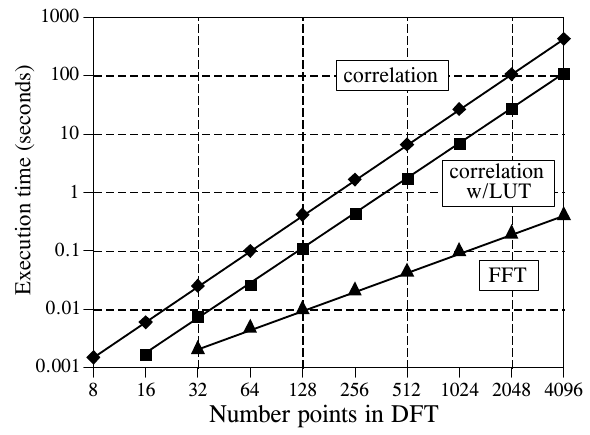
\includegraphics[width=0.492\linewidth,height=0.8\textheight,keepaspectratio]{assets/ch12/fig12-08.png}
\caption*{\textbf{图 12-8　计算 DFT 的执行时间。} 相关法指表 12-2
描述的算法。预先算好正弦和余弦值并存进查找表（LUT），可以让这种方法更快。当
DFT 长于 16 点时，FFT（表 12-3）是最快的算法。图中的时间是在 100 MHz
奔腾处理器上测得的。 （Execution time (seconds) = 执行时间（秒），Number
points in DFT = DFT 的点数；correlation = 相关法，correlation w/LUT =
使用查找表的相关法，FFT = FFT。）}
\end{figure}

FFT 除了速度快，还有另一个优点：因为计算次数少，舍入误差更小，所以 FFT
算得更精确。这可以这样演示：对一个任意信号做 FFT，再把得到的频谱送进逆
FFT。这就重建了原始时域信号，只是多了计算带来的舍入噪声。计算两个信号之差的标准差，就能得到刻画这种噪声的一个数。作为对比，可以用相关法计算的
DFT 及相应的逆 DFT 重复同样的过程。FFT 的舍入噪声与相关法 DFT
相比如何？请看图 12-9。

\begin{figure}[htbp]
\centering
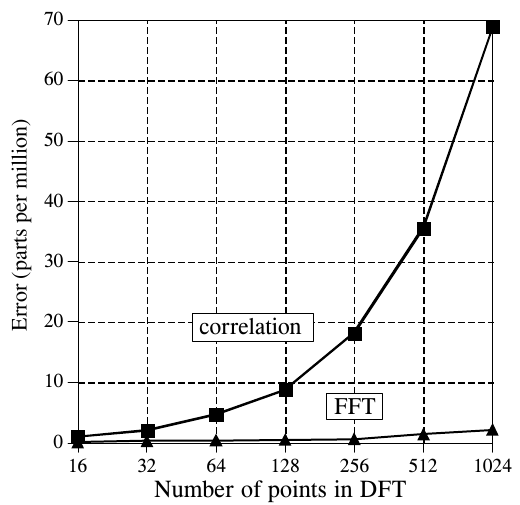
\includegraphics[width=0.433\linewidth,height=0.8\textheight,keepaspectratio]{assets/ch12/fig12-09.png}
\caption*{\textbf{图 12-9　DFT 的精度。} FFT 计算 DFT
比相关法快，同时舍入误差也更小。 （Error (parts per million) =
误差（百万分之一，ppm），Number of points in DFT = DFT
的点数；correlation = 相关法，FFT = FFT。）}
\end{figure}

\texttt{c/table12-5\_inverse\_fft.c}
按上文的方法重做了这个实验：全程单精度，随机信号正变换再逆变换，取原信号与还原信号之差的标准差。实测结果如下（ppm）：

\begingroup\scriptsize\setlength{\tabcolsep}{3pt}

{\def\LTcaptype{none} % do not increment counter
\begin{longtable}[]{@{}llllllll@{}}
\toprule\noalign{}
DFT 点数 & 16 & 32 & 64 & 128 & 256 & 512 & 1024 \\
\midrule\noalign{}
\endhead
\bottomrule\noalign{}
\endlastfoot
FFT & 0.04 & 0.10 & 0.12 & 0.22 & 0.25 & 0.72 & 0.92 \\
相关法 & 0.24 & 0.93 & 2.2 & 3.3 & 8.2 & 14 & 32 \\
\end{longtable}
}

\endgroup

趋势与图 12-9 一致：相关法的误差随 N 快速增长，FFT 一直维持在 1 ppm
左右。具体数值比书上小（书上 1024 点时约 69 ppm 和 2
ppm），这与随机信号的幅度和编译器、浮点库的实现有关。相关法误差大的一个主要原因是它要算
sin(2πki/N)，角度最大接近
2πN，单精度表示这么大的角度本身就有舍入误差；如果先用双精度算好正弦值再转成单精度，两种方法的误差就差不多了。

\section{进一步提速}

有几种技术能让 FFT 更快，不过提升只有 20～40\%
左右。其中一种方法是让时域分解提前两个阶段停下来，此时每个信号只有四个点。不再计算最后两个阶段，而是利用四点正弦、余弦波的简单性，用高度优化的代码直接跳到频域。

另一种流行的算法消除了因时域虚部为零、频谱对称而造成的无用计算。换句话说，把
FFT 修改成计算实数 DFT，而不是复数 DFT。这类算法叫实数 FFT(real FFT)
和实数逆 FFT(real Inverse FFT)（或类似的名字）。可以预期它们比常规 FFT
程序快 30\% 左右。表 12-6 和表 12-7 给出了这两种算法的程序。

\textbf{表 12-6　实数信号的逆 FFT。}（注释已译成中文）

\begin{Shaded}
\begin{Highlighting}[]
\NormalTok{4000 \textquotesingle{}INVERSE FFT FOR REAL SIGNALS}
\NormalTok{4010 \textquotesingle{}进入时，N\% 是 IDFT 的点数，REX[ ] 和}
\NormalTok{4020 \textquotesingle{}IMX[ ] 是频域的实部和虚部，下标从}
\NormalTok{4030 \textquotesingle{}0 到 N\%/2。REX[ ] 和 IMX[ ] 的其余采样被忽略。}
\NormalTok{4040 \textquotesingle{}返回时，REX[ ] 存放实时域信号，IMX[ ] 全为零。}
\NormalTok{4050 \textquotesingle{}}
\NormalTok{4060 \textquotesingle{}}
\NormalTok{4070 FOR K\% = (N\%/2+1) TO (N\%{-}1)                        \textquotesingle{}让频域对称}
\NormalTok{4080 REX[K\%] = REX[N\%{-}K\%]                               \textquotesingle{}（同表 12{-}1）}
\NormalTok{4090 IMX[K\%] = {-}IMX[N\%{-}K\%]}
\NormalTok{4100 NEXT K\%}
\NormalTok{4110 \textquotesingle{}}
\NormalTok{4120 FOR K\% = 0 TO N\%{-}1                                 \textquotesingle{}把实部和虚部相加}
\NormalTok{4130 REX[K\%] = REX[K\%]+IMX[K\%]}
\NormalTok{4140 NEXT K\%}
\NormalTok{4150 \textquotesingle{}}
\NormalTok{4160 GOSUB 3000                                         \textquotesingle{}计算正向实数 DFT（表 12{-}6）}
\NormalTok{4170 \textquotesingle{}}
\NormalTok{4180 FOR I\% = 0 TO N\%{-}1                                 \textquotesingle{}把实部和虚部相加，}
\NormalTok{4190 REX[I\%] = (REX[I\%]+IMX[I\%])/N\%                     \textquotesingle{}并把时域除以 N\%}
\NormalTok{4200 IMX[I\%] = 0}
\NormalTok{4210 NEXT I\%}
\NormalTok{4220 \textquotesingle{}}
\NormalTok{4230 RETURN}
\end{Highlighting}
\end{Shaded}

\begin{quote}
\textbf{译注：} 第 4160 行注释写''表 12-6''，即本表自己；实际调用的第
3000 行子程序是表 12-7 的实数
FFT。另外，``实部加虚部、做正变换、再实部加虚部''之所以能完成逆变换，用的是哈特利变换(Hartley
transform)的性质，原书没有解释。
\end{quote}

\textbf{C 实现}（完整可编译版本见
\texttt{c/table12-6\_real\_inverse\_fft.c}，文件里自带一份表 12-4 的 FFT
和表 12-7 的实数 FFT）：

\begin{Shaded}
\begin{Highlighting}[]
\CommentTok{/* 4000：实数逆 FFT */}
\DataTypeTok{static} \DataTypeTok{void}\NormalTok{ real\_inverse\_fft}\OperatorTok{(}\DataTypeTok{double} \OperatorTok{*}\NormalTok{rex}\OperatorTok{,} \DataTypeTok{double} \OperatorTok{*}\NormalTok{imx}\OperatorTok{,} \DataTypeTok{int}\NormalTok{ n}\OperatorTok{)}
\OperatorTok{\{}
    \ControlFlowTok{for} \OperatorTok{(}\DataTypeTok{int}\NormalTok{ k }\OperatorTok{=}\NormalTok{ n }\OperatorTok{/} \DecValTok{2} \OperatorTok{+} \DecValTok{1}\OperatorTok{;}\NormalTok{ k }\OperatorTok{\textless{}=}\NormalTok{ n }\OperatorTok{{-}} \DecValTok{1}\OperatorTok{;}\NormalTok{ k}\OperatorTok{++)} \OperatorTok{\{}  \CommentTok{/* 4070～4100：让频域对称（同表 12{-}1） */}
\NormalTok{        rex}\OperatorTok{[}\NormalTok{k}\OperatorTok{]} \OperatorTok{=}\NormalTok{ rex}\OperatorTok{[}\NormalTok{n }\OperatorTok{{-}}\NormalTok{ k}\OperatorTok{];}
\NormalTok{        imx}\OperatorTok{[}\NormalTok{k}\OperatorTok{]} \OperatorTok{=} \OperatorTok{{-}}\NormalTok{imx}\OperatorTok{[}\NormalTok{n }\OperatorTok{{-}}\NormalTok{ k}\OperatorTok{];}
    \OperatorTok{\}}

    \ControlFlowTok{for} \OperatorTok{(}\DataTypeTok{int}\NormalTok{ k }\OperatorTok{=} \DecValTok{0}\OperatorTok{;}\NormalTok{ k }\OperatorTok{\textless{}=}\NormalTok{ n }\OperatorTok{{-}} \DecValTok{1}\OperatorTok{;}\NormalTok{ k}\OperatorTok{++)}            \CommentTok{/* 4120～4140：实部和虚部相加 */}
\NormalTok{        rex}\OperatorTok{[}\NormalTok{k}\OperatorTok{]} \OperatorTok{=}\NormalTok{ rex}\OperatorTok{[}\NormalTok{k}\OperatorTok{]} \OperatorTok{+}\NormalTok{ imx}\OperatorTok{[}\NormalTok{k}\OperatorTok{];}

\NormalTok{    real\_fft}\OperatorTok{(}\NormalTok{rex}\OperatorTok{,}\NormalTok{ imx}\OperatorTok{,}\NormalTok{ n}\OperatorTok{);}                      \CommentTok{/* 4160：做正向实数 FFT（原书注释误写为表 12{-}6，实为表 12{-}7） */}

    \ControlFlowTok{for} \OperatorTok{(}\DataTypeTok{int}\NormalTok{ i }\OperatorTok{=} \DecValTok{0}\OperatorTok{;}\NormalTok{ i }\OperatorTok{\textless{}=}\NormalTok{ n }\OperatorTok{{-}} \DecValTok{1}\OperatorTok{;}\NormalTok{ i}\OperatorTok{++)} \OperatorTok{\{}          \CommentTok{/* 4180～4210：实部虚部相加，再除以 N */}
\NormalTok{        rex}\OperatorTok{[}\NormalTok{i}\OperatorTok{]} \OperatorTok{=} \OperatorTok{(}\NormalTok{rex}\OperatorTok{[}\NormalTok{i}\OperatorTok{]} \OperatorTok{+}\NormalTok{ imx}\OperatorTok{[}\NormalTok{i}\OperatorTok{])} \OperatorTok{/}\NormalTok{ n}\OperatorTok{;}
\NormalTok{        imx}\OperatorTok{[}\NormalTok{i}\OperatorTok{]} \OperatorTok{=} \DecValTok{0}\OperatorTok{;}
    \OperatorTok{\}}
\OperatorTok{\}}
\end{Highlighting}
\end{Shaded}

运行结果：随机实信号经实数 FFT 变到频域，只把第 0～N/2 点交给实数逆
FFT（其余点故意写成垃圾值 999），还原结果与原信号最大偏差 N=8 时
1.1e-16，N=64 时 5.3e-16，N=1024 时 1.8e-14。

使用实数 FFT
有两个小缺点。第一，代码长了大约一倍。你的计算机并不在乎，但你得花时间把别人的程序改到自己的机器上运行。第二，调试这些程序稍难一些，因为你不能再用对称性来检查它是否工作正常：这些算法强制时域虚部为零、频域左右对称。调试时，要检查它们的输出与常规
FFT 算法是否一致。

图 12-10 和图 12-11 说明了实数 FFT 的工作原理。在图 12-10 中，(a) 和 (b)
是一个时域信号：实部是一个脉冲，虚部全为零。(c) 和 (d)
是对应的频谱。如前所述，频域的实部关于第 0 个和第 N/2 个采样偶对称(even
symmetry)，虚部关于同样这两点奇对称(odd symmetry)。

\begin{figure}[htbp]
\centering
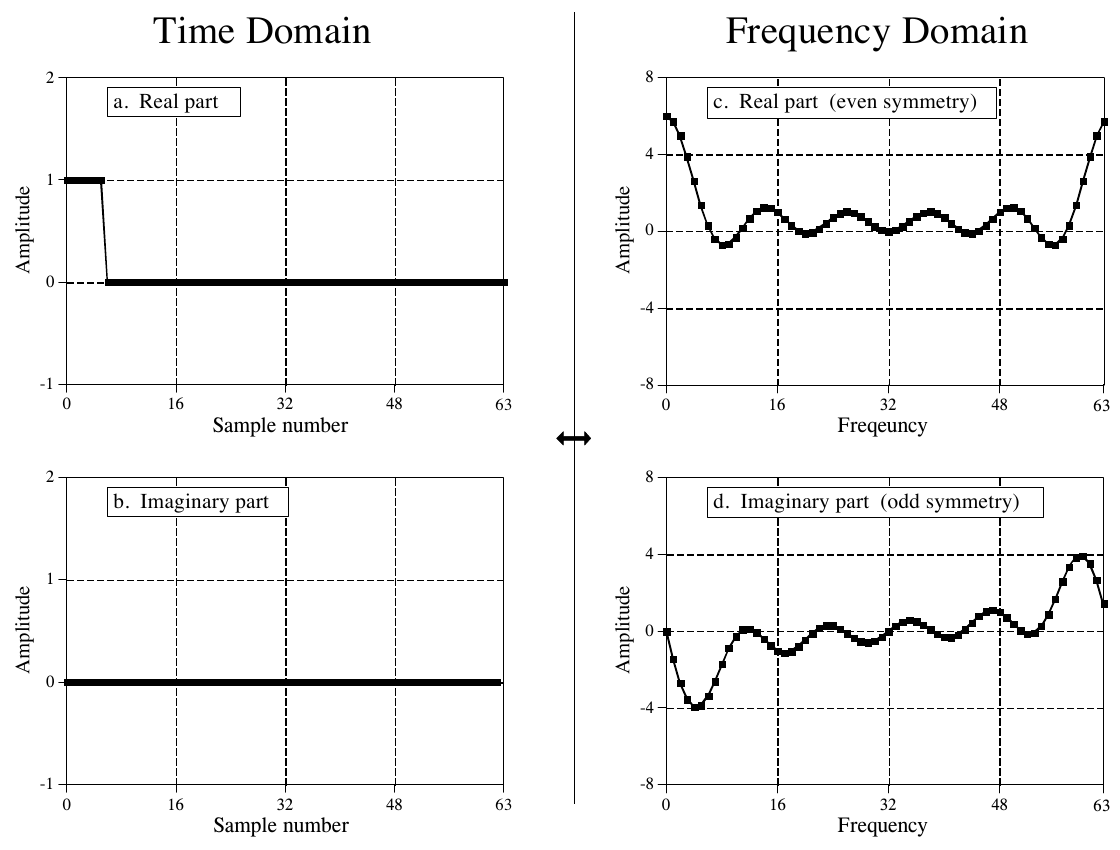
\includegraphics[width=0.933\linewidth,height=0.8\textheight,keepaspectratio]{assets/ch12/fig12-10.png}
\caption*{\textbf{图 12-10　DFT 的实部对称性。} （Time Domain = 时域，Frequency
Domain = 频域；a. Real part = 实部，b. Imaginary part = 虚部，c.~Real
part (even symmetry) = 实部（偶对称），d.~Imaginary part (odd symmetry)
= 虚部（奇对称）。Amplitude = 幅度，Sample number = 采样序号，Frequency
= 频率（(c) 的横轴标注原书误拼为 Freqeuncy）。）}
\end{figure}

再看图
12-11，这时脉冲在时域的虚部，实部全为零。频域的对称性反了过来：实部是奇对称，虚部是偶对称。这种情况将在第
29 章讨论（译注：实为第 31 章）。眼下就先接受复数 DFT 是这样表现的。

\begin{figure}[htbp]
\centering
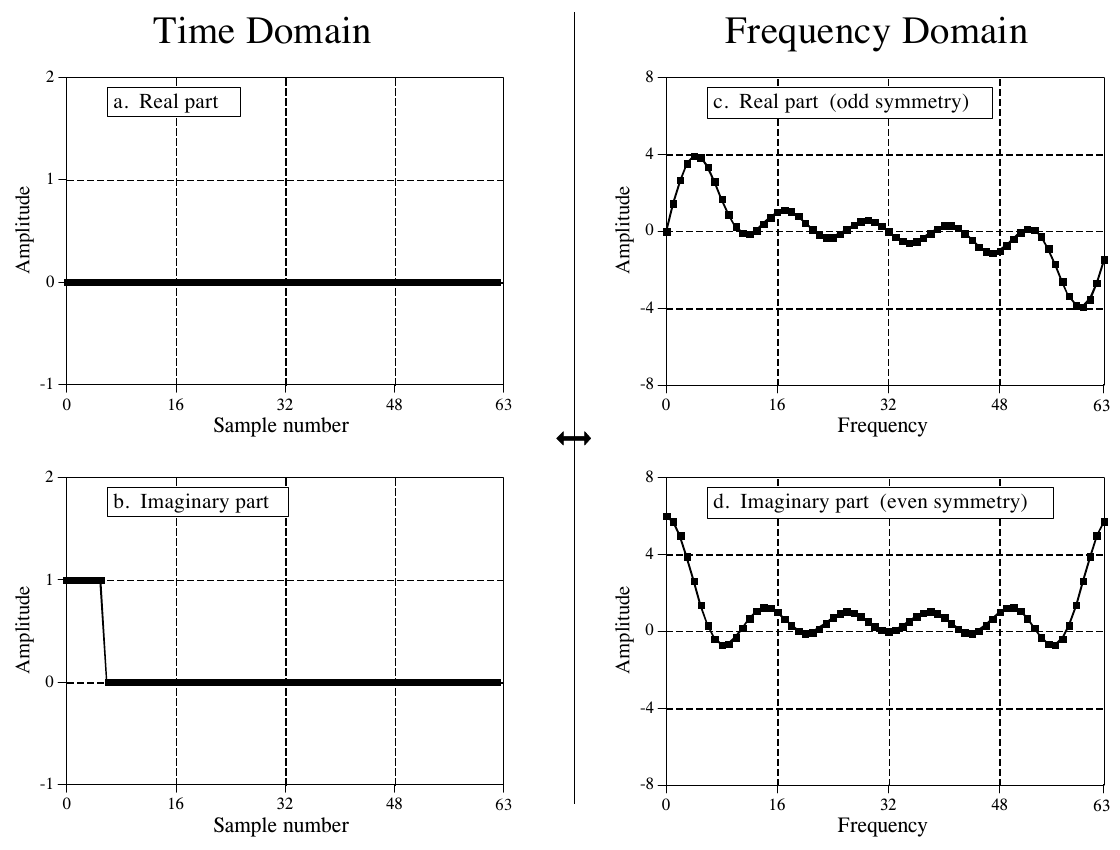
\includegraphics[width=0.933\linewidth,height=0.8\textheight,keepaspectratio]{assets/ch12/fig12-11.png}
\caption*{\textbf{图 12-11　DFT 的虚部对称性。} （a. Real part = 实部，b.
Imaginary part = 虚部，c.~Real part (odd symmetry) =
实部（奇对称），d.~Imaginary part (even symmetry) =
虚部（偶对称）。其余标注同图 12-10。）}
\end{figure}

如果时域的两部分都有信号呢？根据可加性，频域就是两个频谱之和。关键在于：由这两种对称性组成的频谱，可以完美地分离成两个分量信号。这可以用偶/奇分解(even/odd
decomposition)来实现，该方法在第 6 章讨论过（译注：实为第 5
章）。换句话说，花一次 FFT 的代价就能算出两个实数
DFT。把一个信号放进时域实部，另一个信号放进时域虚部。计算复数
DFT（当然是用
FFT）之后，再用偶/奇分解把两个频谱分开。当需要让两个或更多信号通过 FFT
时，这种技术能把执行时间减少约
40\%。之所以达不到整整两倍，是因为偶/奇分解本身也要花计算时间。这是一种相对简单、陷阱很少的技术，完全不像从零写一个
FFT 程序那样难。

下一步是修改算法，让单个 DFT
算得更快。方法很难看，但做法如下。用交错分解把输入信号一分为二：N/2
个偶数点放进时域信号的实部，N/2 个奇数点放进虚部。然后计算一个 N/2 点
FFT，所需时间大约是 N 点 FFT
的一半。再用偶/奇分解把得到的频域分开，得到两个交错时域信号的频谱。最后，像
FFT 的最后一个合成阶段那样，把这两个频谱合并成一个频谱。

作为本章的结尾，不妨这样看：FFT
之于数字信号处理，就像晶体管之于电子学。它是这门技术的基石；这一领域里人人都知道它的特性和用法，但真正懂得其内部工作细节的，只有少数专家。

\textbf{表 12-7　实数信号的 FFT。}（注释已译成中文）

\begin{Shaded}
\begin{Highlighting}[]
\NormalTok{3000 \textquotesingle{}FFT FOR REAL SIGNALS}
\NormalTok{3010 \textquotesingle{}进入时，N\% 是 DFT 的点数，REX[ ] 存放}
\NormalTok{3020 \textquotesingle{}实输入信号，IMX[ ] 中的值被忽略。返回时，}
\NormalTok{3030 \textquotesingle{}REX[ ] 和 IMX[ ] 存放 DFT 的输出。所有信号都从 0 到 N\%{-}1。}
\NormalTok{3040 \textquotesingle{}}
\NormalTok{3050 NH\% = N\%/2{-}1                                   \textquotesingle{}把偶数点和奇数点分开}
\NormalTok{3060 FOR I\% = 0 TO NH\%}
\NormalTok{3070 REX(I\%) = REX(2*I\%)}
\NormalTok{3080 IMX(I\%) = REX(2*I\%+1)}
\NormalTok{3090 NEXT I\%}
\NormalTok{3100 \textquotesingle{}}
\NormalTok{3110 N\% = N\%/2                                      \textquotesingle{}计算 N\%/2 点 FFT}
\NormalTok{3120 GOSUB 1000                                     \textquotesingle{}（GOSUB 1000 是表 12{-}3 的 FFT）}
\NormalTok{3130 N\% = N\%*2}
\NormalTok{3140 \textquotesingle{}}
\NormalTok{3150 NM1\% = N\%{-}1                                    \textquotesingle{}频域的偶/奇分解}
\NormalTok{3160 ND2\% = N\%/2}
\NormalTok{3170 N4\% = N\%/4{-}1}
\NormalTok{3180 FOR I\% = 1 TO N4\%}
\NormalTok{3190 IM\% = ND2\%{-}I\%}
\NormalTok{3200 IP2\% = I\%+ND2\%}
\NormalTok{3210 IPM\% = IM\%+ND2\%}
\NormalTok{3220 REX(IP2\%) = (IMX(I\%) + IMX(IM\%))/2}
\NormalTok{3230 REX(IPM\%) = REX(IP2\%)}
\NormalTok{3240 IMX(IP2\%) = {-}(REX(I\%) {-} REX(IM\%))/2}
\NormalTok{3250 IMX(IPM\%) = {-}IMX(IP2\%)}
\NormalTok{3260 REX(I\%) = (REX(I\%) + REX(IM\%))/2}
\NormalTok{3270 REX(IM\%) = REX(I\%)}
\NormalTok{3280 IMX(I\%) = (IMX(I\%) {-} IMX(IM\%))/2}
\NormalTok{3290 IMX(IM\%) = {-}IMX(I\%)}
\NormalTok{3300 NEXT I\%}
\NormalTok{3310 REX(N\%*3/4) = IMX(N\%/4)}
\NormalTok{3320 REX(ND2\%) = IMX(0)}
\NormalTok{3330 IMX(N\%*3/4) = 0}
\NormalTok{3340 IMX(ND2\%) = 0}
\NormalTok{3350 IMX(N\%/4) = 0}
\NormalTok{3360 IMX(0) = 0}
\NormalTok{3370 \textquotesingle{}}
\NormalTok{3380 PI = 3.14159265                                          \textquotesingle{}补做 FFT 的最后一级}
\NormalTok{3390 L\% = CINT(LOG(N\%)/LOG(2))}
\NormalTok{3400 LE\% = CINT(2\^{}L\%)}
\NormalTok{3410 LE2\% = LE\%/2}
\NormalTok{3420 UR = 1}
\NormalTok{3430 UI = 0}
\NormalTok{3440 SR = COS(PI/LE2\%)}
\NormalTok{3450 SI = {-}SIN(PI/LE2\%)}
\NormalTok{3460 FOR J\% = 1 TO LE2\%}
\NormalTok{3470 JM1\% = J\%{-}1}
\NormalTok{3480 FOR I\% = JM1\% TO NM1\% STEP LE\%}
\NormalTok{3490 IP\% = I\%+LE2\%}
\NormalTok{3500 TR = REX[IP\%]*UR {-} IMX[IP\%]*UI}
\NormalTok{3510 TI = REX[IP\%]*UI + IMX[IP\%]*UR}
\NormalTok{3520 REX[IP\%] = REX[I\%]{-}TR}
\NormalTok{3530 IMX[IP\%] = IMX[I\%]{-}TI}
\NormalTok{3540 REX[I\%] = REX[I\%]+TR}
\NormalTok{3550 IMX[I\%] = IMX[I\%]+TI}
\NormalTok{3560 NEXT I\%}
\NormalTok{3570 TR = UR}
\NormalTok{3580 UR = TR*SR {-} UI*SI}
\NormalTok{3590 UI = TR*SI + UI*SR}
\NormalTok{3600 NEXT J\%}
\NormalTok{3610 RETURN}
\end{Highlighting}
\end{Shaded}

\begin{quote}
\textbf{译注：} 第 3120 行注释写''表 12-3''，实际调用的是表 12-4 的
BASIC 版 FFT。原程序中数组括号 ( ) 和 {[} {]} 混用，含义相同。
\end{quote}

\textbf{C 实现}（完整可编译版本见
\texttt{c/table12-7\_real\_fft.c}，文件里自带一份表 12-4 的 FFT）：

\begin{Shaded}
\begin{Highlighting}[]
\CommentTok{/* 3000：实数 FFT。进入时 rex[] 是实信号（imx[] 内容忽略），返回时 rex/imx 是 0～n{-}1 的完整频谱 */}
\DataTypeTok{static} \DataTypeTok{void}\NormalTok{ real\_fft}\OperatorTok{(}\DataTypeTok{double} \OperatorTok{*}\NormalTok{rex}\OperatorTok{,} \DataTypeTok{double} \OperatorTok{*}\NormalTok{imx}\OperatorTok{,} \DataTypeTok{int}\NormalTok{ n}\OperatorTok{)}
\OperatorTok{\{}
    \DataTypeTok{int}\NormalTok{ nh }\OperatorTok{=}\NormalTok{ n }\OperatorTok{/} \DecValTok{2} \OperatorTok{{-}} \DecValTok{1}\OperatorTok{;}                         \CommentTok{/* 3050：拆开偶数点和奇数点 */}
    \ControlFlowTok{for} \OperatorTok{(}\DataTypeTok{int}\NormalTok{ i }\OperatorTok{=} \DecValTok{0}\OperatorTok{;}\NormalTok{ i }\OperatorTok{\textless{}=}\NormalTok{ nh}\OperatorTok{;}\NormalTok{ i}\OperatorTok{++)} \OperatorTok{\{}             \CommentTok{/* 3060～3090：偶数点进实部，奇数点进虚部 */}
\NormalTok{        rex}\OperatorTok{[}\NormalTok{i}\OperatorTok{]} \OperatorTok{=}\NormalTok{ rex}\OperatorTok{[}\DecValTok{2} \OperatorTok{*}\NormalTok{ i}\OperatorTok{];}                    \CommentTok{/* 从小下标往上写，不会覆盖还没读的点 */}
\NormalTok{        imx}\OperatorTok{[}\NormalTok{i}\OperatorTok{]} \OperatorTok{=}\NormalTok{ rex}\OperatorTok{[}\DecValTok{2} \OperatorTok{*}\NormalTok{ i }\OperatorTok{+} \DecValTok{1}\OperatorTok{];}
    \OperatorTok{\}}

\NormalTok{    fft}\OperatorTok{(}\NormalTok{rex}\OperatorTok{,}\NormalTok{ imx}\OperatorTok{,}\NormalTok{ n }\OperatorTok{/} \DecValTok{2}\OperatorTok{);}                       \CommentTok{/* 3110～3130：做 N/2 点 FFT */}

    \DataTypeTok{int}\NormalTok{ nm1 }\OperatorTok{=}\NormalTok{ n }\OperatorTok{{-}} \DecValTok{1}\OperatorTok{,}\NormalTok{ nd2 }\OperatorTok{=}\NormalTok{ n }\OperatorTok{/} \DecValTok{2}\OperatorTok{,}\NormalTok{ n4 }\OperatorTok{=}\NormalTok{ n }\OperatorTok{/} \DecValTok{4} \OperatorTok{{-}} \DecValTok{1}\OperatorTok{;}   \CommentTok{/* 3150～3170：频域的偶/奇分解 */}
    \ControlFlowTok{for} \OperatorTok{(}\DataTypeTok{int}\NormalTok{ i }\OperatorTok{=} \DecValTok{1}\OperatorTok{;}\NormalTok{ i }\OperatorTok{\textless{}=}\NormalTok{ n4}\OperatorTok{;}\NormalTok{ i}\OperatorTok{++)} \OperatorTok{\{}             \CommentTok{/* 3180：每次处理一对对称点 I 和 N/2{-}I */}
        \DataTypeTok{int}\NormalTok{ im }\OperatorTok{=}\NormalTok{ nd2 }\OperatorTok{{-}}\NormalTok{ i}\OperatorTok{;}                       \CommentTok{/* 3190 */}
        \DataTypeTok{int}\NormalTok{ ip2 }\OperatorTok{=}\NormalTok{ i }\OperatorTok{+}\NormalTok{ nd2}\OperatorTok{;}                      \CommentTok{/* 3200 */}
        \DataTypeTok{int}\NormalTok{ ipm }\OperatorTok{=}\NormalTok{ im }\OperatorTok{+}\NormalTok{ nd2}\OperatorTok{;}                     \CommentTok{/* 3210 */}
\NormalTok{        rex}\OperatorTok{[}\NormalTok{ip2}\OperatorTok{]} \OperatorTok{=} \OperatorTok{(}\NormalTok{imx}\OperatorTok{[}\NormalTok{i}\OperatorTok{]} \OperatorTok{+}\NormalTok{ imx}\OperatorTok{[}\NormalTok{im}\OperatorTok{])} \OperatorTok{/} \DecValTok{2}\OperatorTok{;}      \CommentTok{/* 3220～3250：奇数点信号的频谱，放在后半段 */}
\NormalTok{        rex}\OperatorTok{[}\NormalTok{ipm}\OperatorTok{]} \OperatorTok{=}\NormalTok{ rex}\OperatorTok{[}\NormalTok{ip2}\OperatorTok{];}
\NormalTok{        imx}\OperatorTok{[}\NormalTok{ip2}\OperatorTok{]} \OperatorTok{=} \OperatorTok{{-}(}\NormalTok{rex}\OperatorTok{[}\NormalTok{i}\OperatorTok{]} \OperatorTok{{-}}\NormalTok{ rex}\OperatorTok{[}\NormalTok{im}\OperatorTok{])} \OperatorTok{/} \DecValTok{2}\OperatorTok{;}
\NormalTok{        imx}\OperatorTok{[}\NormalTok{ipm}\OperatorTok{]} \OperatorTok{=} \OperatorTok{{-}}\NormalTok{imx}\OperatorTok{[}\NormalTok{ip2}\OperatorTok{];}
\NormalTok{        rex}\OperatorTok{[}\NormalTok{i}\OperatorTok{]} \OperatorTok{=} \OperatorTok{(}\NormalTok{rex}\OperatorTok{[}\NormalTok{i}\OperatorTok{]} \OperatorTok{+}\NormalTok{ rex}\OperatorTok{[}\NormalTok{im}\OperatorTok{])} \OperatorTok{/} \DecValTok{2}\OperatorTok{;}        \CommentTok{/* 3260～3290：偶数点信号的频谱，留在前半段 */}
\NormalTok{        rex}\OperatorTok{[}\NormalTok{im}\OperatorTok{]} \OperatorTok{=}\NormalTok{ rex}\OperatorTok{[}\NormalTok{i}\OperatorTok{];}
\NormalTok{        imx}\OperatorTok{[}\NormalTok{i}\OperatorTok{]} \OperatorTok{=} \OperatorTok{(}\NormalTok{imx}\OperatorTok{[}\NormalTok{i}\OperatorTok{]} \OperatorTok{{-}}\NormalTok{ imx}\OperatorTok{[}\NormalTok{im}\OperatorTok{])} \OperatorTok{/} \DecValTok{2}\OperatorTok{;}
\NormalTok{        imx}\OperatorTok{[}\NormalTok{im}\OperatorTok{]} \OperatorTok{=} \OperatorTok{{-}}\NormalTok{imx}\OperatorTok{[}\NormalTok{i}\OperatorTok{];}
    \OperatorTok{\}}
\NormalTok{    rex}\OperatorTok{[}\NormalTok{n }\OperatorTok{*} \DecValTok{3} \OperatorTok{/} \DecValTok{4}\OperatorTok{]} \OperatorTok{=}\NormalTok{ imx}\OperatorTok{[}\NormalTok{n }\OperatorTok{/} \DecValTok{4}\OperatorTok{];}                \CommentTok{/* 3310～3360：自身对称的 0 和 N/4 两点单独处理 */}
\NormalTok{    rex}\OperatorTok{[}\NormalTok{nd2}\OperatorTok{]} \OperatorTok{=}\NormalTok{ imx}\OperatorTok{[}\DecValTok{0}\OperatorTok{];}
\NormalTok{    imx}\OperatorTok{[}\NormalTok{n }\OperatorTok{*} \DecValTok{3} \OperatorTok{/} \DecValTok{4}\OperatorTok{]} \OperatorTok{=} \DecValTok{0}\OperatorTok{;}
\NormalTok{    imx}\OperatorTok{[}\NormalTok{nd2}\OperatorTok{]} \OperatorTok{=} \DecValTok{0}\OperatorTok{;}
\NormalTok{    imx}\OperatorTok{[}\NormalTok{n }\OperatorTok{/} \DecValTok{4}\OperatorTok{]} \OperatorTok{=} \DecValTok{0}\OperatorTok{;}
\NormalTok{    imx}\OperatorTok{[}\DecValTok{0}\OperatorTok{]} \OperatorTok{=} \DecValTok{0}\OperatorTok{;}

    \DataTypeTok{int}\NormalTok{ l }\OperatorTok{=} \OperatorTok{(}\DataTypeTok{int}\OperatorTok{)}\NormalTok{lround}\OperatorTok{(}\NormalTok{log}\OperatorTok{(}\NormalTok{n}\OperatorTok{)} \OperatorTok{/}\NormalTok{ log}\OperatorTok{(}\DecValTok{2}\OperatorTok{));}       \CommentTok{/* 3380～3600：补做 FFT 的最后一级 */}
    \DataTypeTok{int}\NormalTok{ le }\OperatorTok{=} \DecValTok{1} \OperatorTok{\textless{}\textless{}}\NormalTok{ l}\OperatorTok{;}                            \CommentTok{/* 3400：最后一级 LE = N */}
    \DataTypeTok{int}\NormalTok{ le2 }\OperatorTok{=}\NormalTok{ le }\OperatorTok{/} \DecValTok{2}\OperatorTok{;}
    \DataTypeTok{double}\NormalTok{ ur }\OperatorTok{=} \FloatTok{1.0}\OperatorTok{,}\NormalTok{ ui }\OperatorTok{=} \FloatTok{0.0}\OperatorTok{,}\NormalTok{ sr }\OperatorTok{=}\NormalTok{ cos}\OperatorTok{(}\NormalTok{PI }\OperatorTok{/}\NormalTok{ le2}\OperatorTok{),}\NormalTok{ si }\OperatorTok{=} \OperatorTok{{-}}\NormalTok{sin}\OperatorTok{(}\NormalTok{PI }\OperatorTok{/}\NormalTok{ le2}\OperatorTok{);}
    \ControlFlowTok{for} \OperatorTok{(}\DataTypeTok{int}\NormalTok{ j }\OperatorTok{=} \DecValTok{1}\OperatorTok{;}\NormalTok{ j }\OperatorTok{\textless{}=}\NormalTok{ le2}\OperatorTok{;}\NormalTok{ j}\OperatorTok{++)} \OperatorTok{\{}            \CommentTok{/* 3460 */}
        \DataTypeTok{int}\NormalTok{ jm1 }\OperatorTok{=}\NormalTok{ j }\OperatorTok{{-}} \DecValTok{1}\OperatorTok{;}
        \ControlFlowTok{for} \OperatorTok{(}\DataTypeTok{int}\NormalTok{ i }\OperatorTok{=}\NormalTok{ jm1}\OperatorTok{;}\NormalTok{ i }\OperatorTok{\textless{}=}\NormalTok{ nm1}\OperatorTok{;}\NormalTok{ i }\OperatorTok{+=}\NormalTok{ le}\OperatorTok{)} \OperatorTok{\{}  \CommentTok{/* 3480：最后一级每个 J 只有一个蝶形 */}
            \DataTypeTok{int}\NormalTok{ ip }\OperatorTok{=}\NormalTok{ i }\OperatorTok{+}\NormalTok{ le2}\OperatorTok{;}
            \DataTypeTok{double}\NormalTok{ tr }\OperatorTok{=}\NormalTok{ rex}\OperatorTok{[}\NormalTok{ip}\OperatorTok{]} \OperatorTok{*}\NormalTok{ ur }\OperatorTok{{-}}\NormalTok{ imx}\OperatorTok{[}\NormalTok{ip}\OperatorTok{]} \OperatorTok{*}\NormalTok{ ui}\OperatorTok{;}    \CommentTok{/* 3500～3550：蝶形运算 */}
            \DataTypeTok{double}\NormalTok{ ti }\OperatorTok{=}\NormalTok{ rex}\OperatorTok{[}\NormalTok{ip}\OperatorTok{]} \OperatorTok{*}\NormalTok{ ui }\OperatorTok{+}\NormalTok{ imx}\OperatorTok{[}\NormalTok{ip}\OperatorTok{]} \OperatorTok{*}\NormalTok{ ur}\OperatorTok{;}
\NormalTok{            rex}\OperatorTok{[}\NormalTok{ip}\OperatorTok{]} \OperatorTok{=}\NormalTok{ rex}\OperatorTok{[}\NormalTok{i}\OperatorTok{]} \OperatorTok{{-}}\NormalTok{ tr}\OperatorTok{;}
\NormalTok{            imx}\OperatorTok{[}\NormalTok{ip}\OperatorTok{]} \OperatorTok{=}\NormalTok{ imx}\OperatorTok{[}\NormalTok{i}\OperatorTok{]} \OperatorTok{{-}}\NormalTok{ ti}\OperatorTok{;}
\NormalTok{            rex}\OperatorTok{[}\NormalTok{i}\OperatorTok{]} \OperatorTok{=}\NormalTok{ rex}\OperatorTok{[}\NormalTok{i}\OperatorTok{]} \OperatorTok{+}\NormalTok{ tr}\OperatorTok{;}
\NormalTok{            imx}\OperatorTok{[}\NormalTok{i}\OperatorTok{]} \OperatorTok{=}\NormalTok{ imx}\OperatorTok{[}\NormalTok{i}\OperatorTok{]} \OperatorTok{+}\NormalTok{ ti}\OperatorTok{;}
        \OperatorTok{\}}
        \DataTypeTok{double}\NormalTok{ tr }\OperatorTok{=}\NormalTok{ ur}\OperatorTok{;}                         \CommentTok{/* 3570～3590 */}
\NormalTok{        ur }\OperatorTok{=}\NormalTok{ tr }\OperatorTok{*}\NormalTok{ sr }\OperatorTok{{-}}\NormalTok{ ui }\OperatorTok{*}\NormalTok{ si}\OperatorTok{;}
\NormalTok{        ui }\OperatorTok{=}\NormalTok{ tr }\OperatorTok{*}\NormalTok{ si }\OperatorTok{+}\NormalTok{ ui }\OperatorTok{*}\NormalTok{ sr}\OperatorTok{;}
    \OperatorTok{\}}
\OperatorTok{\}}
\end{Highlighting}
\end{Shaded}

运行结果： - 随机实信号用实数 FFT 计算，与普通复数 FFT（虚部填
0）逐点比较，最大偏差 N=8 时 1.1e-16，N=64 时 1.8e-15，N=1024 时
1.2e-13。进入时故意在 IMX{[} {]} 里填了垃圾值，确认它确实被忽略。 - 1024
点各算 20000 次：复数 FFT 154 ms，实数 FFT 80
ms。这台机器上快了约一倍，比书上说的 30\% 还多。
